\documentclass[12pt]{book}

\usepackage{tikz} 
\usepackage{tikz-network}
\usepackage{graphics}
\usepackage{graphicx}
\usetikzlibrary{automata} 
\usetikzlibrary{positioning} 
\usetikzlibrary{arrows} 
\usepackage{hyperref}
\hypersetup{
    colorlinks=true, %set true if you want colored links
    linktoc=all,     %set to all if you want both sections and subsections linked
    linkcolor=black,  %choose some color if you want links to stand out
}
\usepackage{amsmath, amssymb}
\tikzset{node distance=2.5cm, 
every state/.style={ % Sets the properties for each state
semithick,
fill=gray!10},
initial text={}, % No label on start arrow
double distance=2pt, % Adjust appearance of accept states
every edge/.style={ % Sets the properties for each transition
draw,
->, % Makes edges directed with bold arrowheads
auto,
semithick}}
\let\epsilon\varepsilon


%\renewcommand{\baselinestretch}{1.3} 

\begin{document}

\tableofcontents

\chapter{Finite Automata}

In This Book We Learn :

\begin{enumerate}
	\item The Theory Of Automata
	\item Formal Languages
	\item Regular Sets and Regular Grammars
	\item Context Free Languages
	\item Pushdown Automata
	\item LR(K) Grammars
	\item Turing Machine
\end{enumerate}


\section{Definition of Finite Automata}

F.A. can be represented by a 5-tuple $(Q,\Sigma,\delta,q_{0},F)$ where :

\begin{itemize}
	\item Q is finite non-empty set of states
	\item $\Sigma$ is finite non-empty set of input alphabets
	\item $\delta$ is the transition function which maps : $Q \times \Sigma \to Q$
	\item $q_{0} \in Q$ is the initial state 
	\item $F \subseteq Q$ is the set of final states
\end{itemize}


\section{Example of lift control}


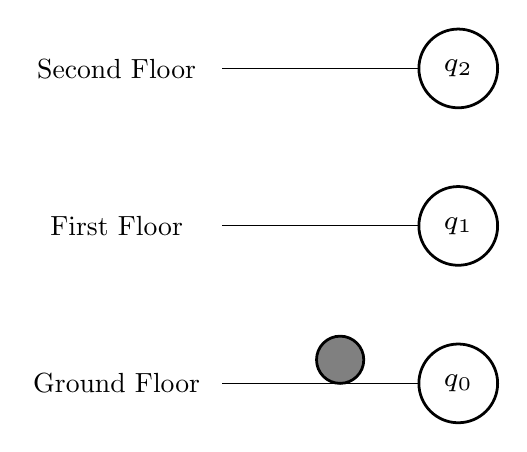
\begin{tikzpicture}
\draw (0,0) to (3,0);
\draw (0,2) to (3,2);
\draw (0,4) to (3,4);
\Text[x=-1.3,y=0]{Ground Floor\:}
\Text[x=-1.3,y=2]{First Floor\:}
\Text[x=-1.3,y=4]{Second Floor\:}
\Vertex[x=1.5,y=0.3,color = gray]{BOX}
\Vertex[x=3,y=0,label=$q_0$,color=white,size=1,fontscale=1.4]{A}
\Vertex[x=3,y=2,label=$q_1$,color=white,size=1,fontscale=1.4]{B}
\Vertex[x=3,y=4,label=$q_2$,color=white,size=1,fontscale=1.4]{C}
\end{tikzpicture}


$$
Q = \{ q_{0} , q_{1} , q_{2} \}
$$

$$
\Sigma = \{ 0 , 1 , 2 \}
$$

$$
q_{0} = initial \:\: state , q_{0} \in Q
$$

$$
F = \{ q_{2} \}  \subseteq Q
$$


\begin{tabular}{l | c  c  c } 
\multicolumn{4}{ c }{Transition Table} \\
               & 0 & 1 & 2  \\
\hline
$q_{0}$ & $q_{0}$ & $q_{1}$ & $q_{2}$   \\
$q_{1}$ & $q_{0}$ & $q_{1}$ & $q_{2}$   \\
$q_{2}$ & $q_{0}$ & $q_{1}$ & $q_{2}$   \\
\end{tabular}


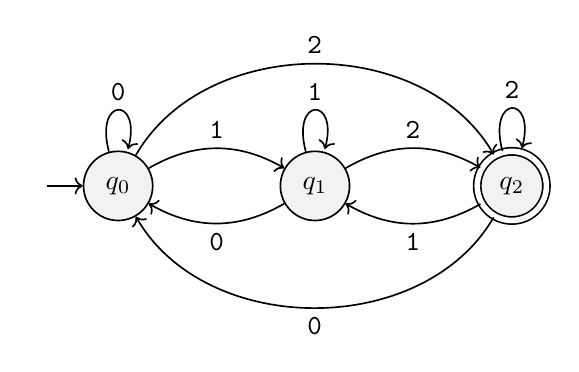
\begin{tikzpicture}
\node[state, initial] (q1) {$q_0$};
\node[state,  right of=q1] (q2) {$q_1$};
\node[state, accepting, right of=q2] (q3) {$q_2$};
\draw (q1) edge[loop above] node {\tt 0} (q1);
\draw (q1) edge[bend left] node {\tt 1} (q2);
\draw (q1) edge[bend left=60] node {\tt 2} (q3);
\draw (q2) edge[loop above] node {\tt 1} (q2);
\draw (q2) edge[bend left] node {\tt 0} (q1);
\draw (q2) edge[bend left] node {\tt 2} (q3);
\draw (q3) edge[bend left=60] node {\tt 0} (q1);
\draw (q3) edge[bend left] node {\tt 1} (q2);
\draw (q3) edge[loop above] node {\tt 2} (q3);
\end{tikzpicture}



\section{Acceptability of a string by DFA}

A string $x \in \Sigma^{*}$ is accepted by a Finite automaton $M = (Q, \Sigma, \delta, q_{0}, F)$ if $\delta(q_{0} , x) = q$ for some $q \in F$.


\section{Properties of Transition Function}

\begin{enumerate}
	\item $\delta(q, \wedge) = q$
	\item For all strings $\omega \in Z^{*}$ and input symbol a :
	
	$$
	\delta(q , a\omega) = \delta( \delta(q,a) , \omega )
	$$
	
	$$
	\delta(q , \omega a) = \delta( \delta(q,\omega) , a )
	$$
\end{enumerate}



\subsection{Example}

Transition table given below, is string 110101 accepted by this machine ?


\begin{tabular}{l | c  c  } 
\multicolumn{3}{ c }{Transition Table} \\
               & $x = 0$ & $x = 1$  \\
\hline
$q_{1}$ & $q_{3}$ & $q_{1}$   \\
$q_{2}$ & $q_{4}$ & $q_{1}$   \\
$q_{3}$ & $q_{1}$ & $q_{4}$   \\
$q_{4}$ & $q_{2}$ & $q_{3}$   \\
\end{tabular}

Answer : Yes, because 

\begin{equation*}
\begin{split} \label{x5}
\delta( q_{1} , \underbrace{1}_{a}\underbrace{10101}_{\omega} ) &= \delta( q_{2} , 10101 ) \\
&= \delta( q_{1} , 0101 ) \\
&= \delta( q_{3} , 101 ) \\
&= \delta( q_{4} , 01 ) \\
&= \delta( q_{2} , 1 ) \\
&= \delta( q_{1} , \wedge ) \\
&= q_{1}
\end{split}
\end{equation*}

so the string is accepted .



\section{Definition of NFA}

A Non-deterministic Finite Automata (NDFA or NFA) is a 5-tuple $(Q, \Sigma, \delta, q_{0}, F)$ where :

\begin{itemize}
	\item Q is a finite non-empty set of states
	\item $\Sigma$ is a finite non-empty set of input alphabets
	\item $\delta$ is the transition function mapping from $Q \times \Sigma \to 2^{Q}$, where $2^{Q}$ is the power-set of all subsets of Q
	\item $q_{0} \in Q$ is the initial state
	\item $F \subseteq Q$ is the set of final states
\end{itemize}


\section{Acceptability by NFA}

A string $\omega \in \Sigma^{*}$ is accepted by NFA $M$ if $\delta(q_{0}, \omega)$ contains some final state.

The set accepted by an automaton M(Deterministic or Non-Deterministic) is the set of all input strings accepted by M. It is denoted by T(M) .

\subsection{Example}

Is the input string 0100 is accepted by NFA below :


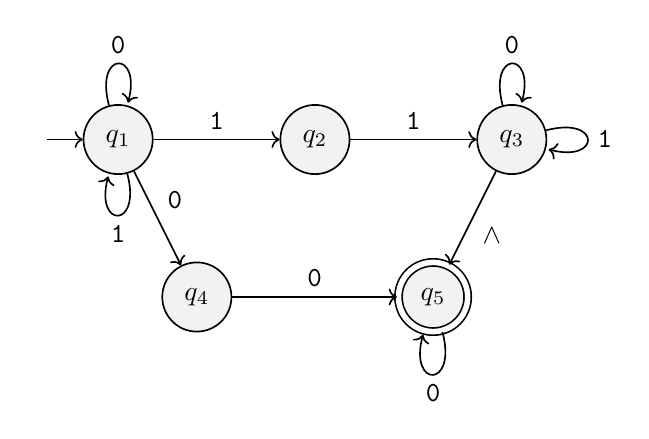
\begin{tikzpicture}
\node[state, initial] (q1) at (0,0) {$q_{1}$};
\node[state] (q2) at (2.5,0) {$q_{2}$};
\node[state] (q3) at (5,0) {$q_{3}$};
\node[state] (q4) at (1,-2) {$q_{4}$};
\node[state, accepting] (q5) at (4,-2) {$q_{5}$};
\draw (q1) edge[loop above] node{\tt 0} (q1);
\draw (q1) edge[loop below] node{\tt 1} (q1);
\draw (q1) edge node{\tt 0} (q4);
\draw (q1) edge node{\tt 1} (q2);
\draw (q2) edge node{\tt 1} (q3);
\draw (q3) edge[loop above] node{\tt 0} (q3);
\draw (q3) edge[loop right] node{\tt 1} (q3);
\draw (q3) edge node{\tt $\wedge$} (q5);
\draw (q4) edge node{\tt 0} (q5);
\draw (q5) edge[loop below] node{\tt 0} (q5);
\end{tikzpicture}



\begin{tikzpicture}
\node {$q_{1}$}
child {node {$q_{4}$}}
child {node {$q_{1}$}
	child {node {$q_{2}$}}
	child {node {$q_{1}$}
		child {node {$q_{1}$}
				child {node {$q_{1}$}}
				child {node {$q_{4}$}}
		}
		child {node {$q_{4}$}
			child {node {$q_{5}$}}
		}
	}
};
\end{tikzpicture}

$q_{5} \in F$ so the string is accepted


\subsection{Example}

Design a DFA which take 0s and 1s as input strings and accepts that string which will have even number of 0s and odd number of 1s ?

EO : Even Number of 0's - Odd Number of 1's


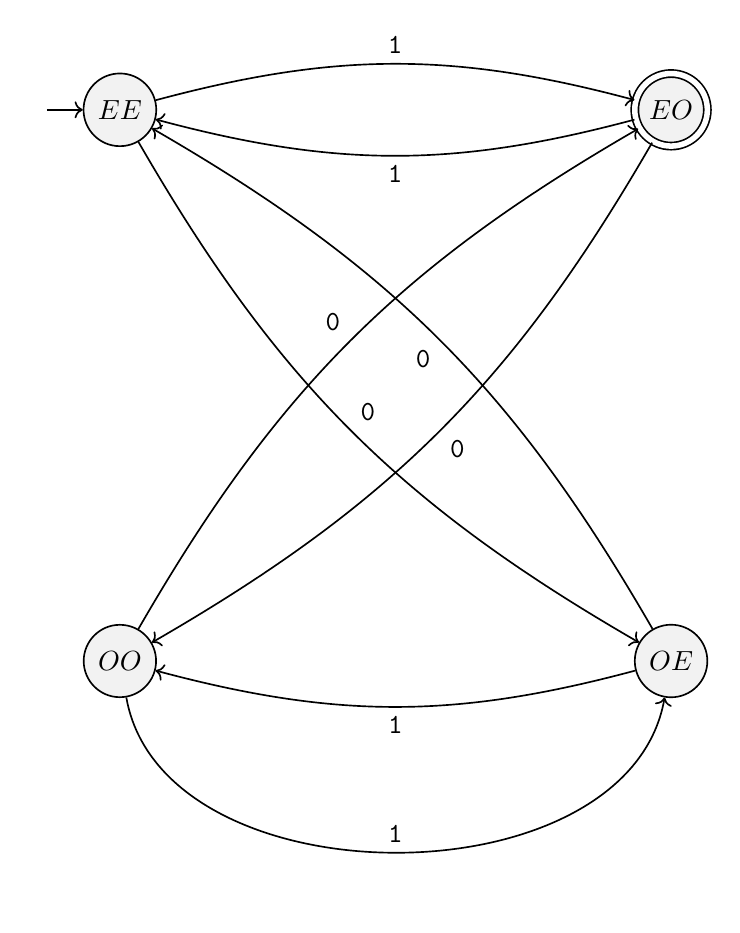
\begin{tikzpicture}
\node[state, initial] (ee) at (0,0) {$EE$};
\node[state, accepting] (eo) at (7,0) {$EO$};
\node[state] (oo) at (0,-7) {$OO$};
\node[state] (oe) at (7,-7) {$OE$};
\draw (ee) edge[bend left=15] node{\tt 1} (eo);
\draw (ee) edge[bend right=15] node{\tt 0} (oe);
\draw (eo) edge[bend left=15] node{\tt 1} (ee);
\draw (eo) edge[bend left=15] node{\tt 0} (oo);
\draw (oe) edge[bend right=15] node{\tt 0} (ee);
\draw (oe) edge[bend left=15] node{\tt 1} (oo);
\draw (oo) edge[bend left=15] node{\tt 0} (eo);
\draw (oo) edge[bend right=80] node{\tt 1} (oe);
\end{tikzpicture}

Suppose :

$$EE \to q_{0}$$
$$OO \to q_{1}$$
$$OE \to q_{2}$$
$$EO \to q_{3}$$



\begin{tabular}{r | c  c  } 
\multicolumn{3}{ c }{Transition Table} \\
               & $x = 0$ & $x = 1$  \\
\hline
$\to q_{0}$ & $q_{2}$ & $q_{3}$   \\
$q_{1}$ & $q_{3}$ & $q_{2}$   \\
$q_{2}$ & $q_{0}$ & $q_{1}$   \\
$(f) \: q_{3}$ & $q_{1}$ & $q_{0}$   \\
\end{tabular}



\subsection{Example}

Design one DFA which Takes 0s and 1s as input string and accepts that binary number which is divisible by 3 ?


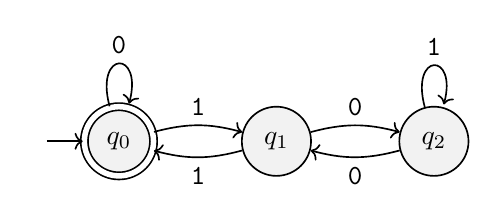
\begin{tikzpicture}
\node[state, initial, accepting] (q0) at (0,0) {$q_{0}$};
\node[state] (q1) at (2,0) {$q_{1}$};
\node[state] (q2) at (4,0) {$q_{2}$};
\draw (q0) edge[loop above] node{\tt 0} (q0);
\draw (q0) edge[bend left=15] node{\tt 1} (q1);
\draw (q1) edge[bend left=15] node{\tt 1} (q0);
\draw (q1) edge[bend left=15] node{\tt 0} (q2);
\draw (q2) edge[bend left=15] node{\tt 0} (q1);
\draw (q2) edge[loop above] node{\tt 1} (q2);
\end{tikzpicture}

We Suppose :


\begin{tabular}{ c |  c |  c  } 
\multicolumn{3}{ c }{} \\
$q_{0} \equiv ( \% 3 == 0 )$ 
& $q_{1} \equiv ( \% 3 == 1 )$ 
& $q_{2} \equiv ( \% 3 == 2 )$  \\
\hline
$0$ & $1$ & $10$   \\
$11$ & $100$ & $101$   \\
$110$ & $111$ & $1000$   \\
$1001$ & $1010$ & $1011$   \\
\end{tabular}




\begin{tabular}{r | c  c  } 
\multicolumn{3}{ c }{} \\
               & $x = 0$ & $x = 1$  \\
\hline
$(f) \to q_{0}$ & $q_{0}$ & $q_{1}$   \\
$q_{1}$ & $q_{2}$ & $q_{0}$   \\
$q_{2}$ & $q_{1}$ & $q_{2}$   \\
\end{tabular}



\section{NFA to DFA Conversion}

Construct a DFA equivalent to 
$M = (\{q_{1},q_{2},q_{3},q_{4}\},\{0,1\},\delta,q_{1},\{q_{4}\})$ where $\delta$ is given below :

\begin{tabular}{r | c  c  } 
\multicolumn{3}{ c }{} \\
               & $0$ & $1$  \\
\hline
$\to q_{1}$ & $q_{1},q_{2}$ & $q_{1}$   \\
$q_{2}$ & $q_{3}$ & $q_{2}$   \\
$q_{3}$ & $q_{4}$ & $q_{4}$   \\
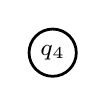
\begin{tikzpicture}\Vertex[x=0,y=0,color=white,label=$q_{4}$,fontscale=1.2]{$q_{4}$}\end{tikzpicture} & $-$ & $q_{3}$   \\
\end{tabular}


Answer :


\begin{tabular}{r | r  r  } 
\multicolumn{3}{ c }{} \\
               & $0$ & $1$  \\
\hline
$\to [q_{1}]$ & $[q_{1},q_{2}]$ & $[q_{1}]$   \\
$[q_{1},q_{2}]$ & $[q_{1},q_{2},q_{3}]$ & $[q_{1},q_{2}]$   \\
$[q_{1},q_{2},q_{3}]$ & $[q_{1},q_{2},q_{3},q_{4}]$ & $[q_{1},q_{2},q_{4}]$   \\
(f)$[q_{1},q_{2},q_{3},q_{4}]$ & $[q_{1},q_{2},q_{3},q_{4}]$ & $[q_{1},q_{2},q_{3},q_{4}]$   \\
(f)$[q_{1},q_{2},q_{4}]$ & $[q_{1},q_{2},q_{3}]$ & $[q_{1},q_{2},q_{3}]$\\
\end{tabular}

note : $q_{4}$ is the final state so every where $q_{4}$ is in the set is the final state .


\section{NFA to DFA Conversion}
Construct a DFA against the following NFA :


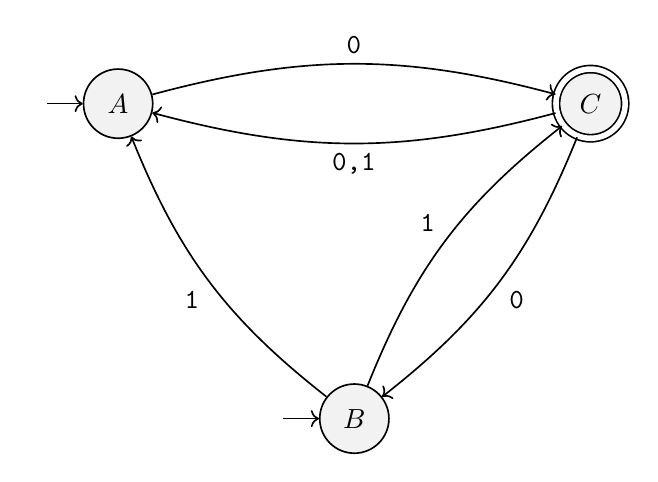
\begin{tikzpicture}
\node[state, initial] (A) at (0,0) {$A$};
\node[state, initial] (B) at (3,-4) {$B$};
\node[state, accepting] (C) at (6,0) {$C$};
\draw (A) edge[bend left=15] node{\tt 0} (C);
\draw (C) edge[bend left=15] node{\tt 0,1} (A);
\draw (B) edge[bend left=15] node{\tt 1} (C);
\draw (C) edge[bend left=15] node{\tt 0} (B);
\draw (B) edge[bend left=15] node{\tt 1} (A);
\end{tikzpicture}


Answer : let's create the transition table :


\begin{tabular}{r | c  c  } 
\multicolumn{3}{ c }{} \\
               & $0$ & $1$  \\
\hline
$\to A$ & $C$ & $-$   \\
$\to B$ & $-$ & $AC$   \\
$(f) C$ & $AB$ & $A$   \\
\end{tabular}


Now let's create Transition table for DFA :

\begin{tabular}{r | r  r  } 
\multicolumn{3}{ c }{} \\
               & $0$ & $1$  \\
\hline
$\to AB$ & $C$ & $AC$   \\
$(f) C$ & $AB$ & $A$   \\
$(f) AC$ & $ABC$ & $A$   \\
$A$ & $C$ & $\phi$   \\
$(f) ABC$ & $ABC$ & $AC$   \\
$\phi$ & $\phi$ & $\phi$   \\
\end{tabular}

note : for initial state we combine all the initial states


and here is the transition diagram for DFA :


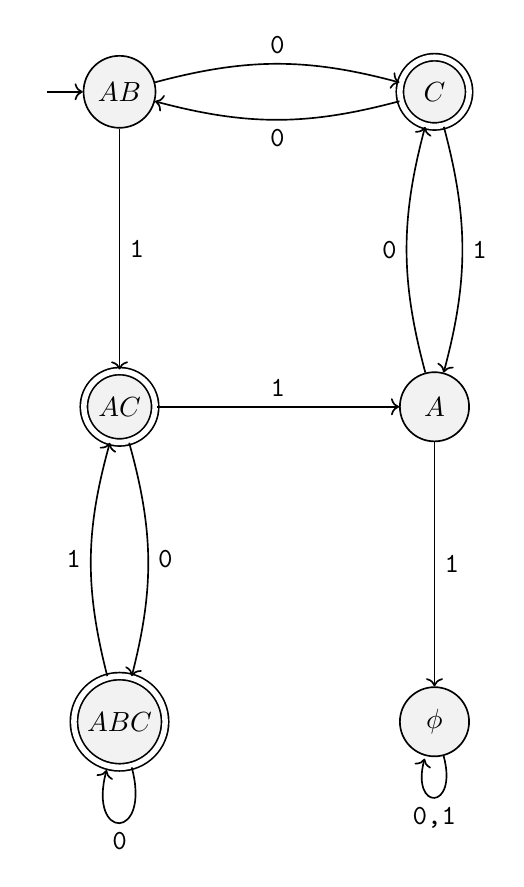
\begin{tikzpicture}
\node[state, initial] (AB) at (0,0) {$AB$};
\node[state, accepting] (C) at (4,0) {$C$};
\node[state, accepting] (AC) at (0,-4) {$AC$};
\node[state] (A) at (4,-4) {$A$};
\node[state, accepting] (ABC) at (0,-8) {$ABC$};
\node[state] (phi) at (4,-8) {$\phi$};
\draw (AB) edge[bend left=15] node{\tt 0} (C);
\draw (C) edge[bend left=15] node{\tt 0} (AB);
\draw (C) edge[bend left=15] node{\tt 1} (A);
\draw (A) edge[bend left=15] node{\tt 0} (C);
\draw (AB) edge node{\tt 1} (AC);
\draw (AC) edge node{\tt 1} (A);
\draw (A) edge node{\tt 1} (phi);
\draw (phi) edge[loop below] node{\tt 0,1} (phi);
\draw (ABC) edge[loop below] node{\tt 0} (ABC);
\draw (ABC) edge[bend left=15] node{\tt 1} (AC);
\draw (AC) edge[bend left=15] node{\tt 0} (ABC);
\end{tikzpicture}


\section{Mealy Machine}

a Mealy Machine is a 6-tuple $(Q, \Sigma, \Delta, \delta, \lambda, q_{0})$, where :

\begin{itemize}
	\item $Q$ is a finite set of states
	\item $\Sigma$ is the set of input alphabets
	\item $\Delta$ is the set of output alphabets
	\item $\delta$ is the transition function $Q \times \Sigma \to Q$
	\item $\lambda$ is the output function mapping $Q \times \Sigma \to \Delta$
	\item $q_{0}$ is the initial state, $q_{0} \in Q$
\end{itemize}

and :
$$
Z(t) = \lambda( q(t), x(t) )
$$
which Z is the output, $\lambda$ is the output function, $q(t)$ is the present state, $x(t)$ is the present input


\subsection{Example of Mealy Machine}

\begin{tabular}{r | c c | c c  } 
& \multicolumn{2}{ c }{$a = 0$} & \multicolumn{2}{ c }{$a = 1$} \\
        & $state$ & $output$ & $state$ & $output$ \\
\hline
$\to q_{0}$ & $q_{2}$ & $0$ & $q_{3}$ & $0$  \\
$q_{1}$ & $q_{3}$ & $1$ & $q_{3}$ & $0$   \\
$q_{2}$ & $q_{0}$ & $1$ & $q_{2}$ & $1$   \\
$q_{3}$ & $q_{1}$ & $0$ & $q_{1}$ & $0$   \\
\end{tabular}


$$
Q = \{ q_{0}, q_{1}, q_{2}, q_{3} \}
$$

$$
\Sigma = \{ 0, 1 \}
$$

$$
\Delta = \{ 0, 1 \}
$$



\section{Moore Machine}

a Moore Machine is a 6-tuple $(Q, \Sigma, \Delta, \delta, \lambda, q_{0})$, where :

\begin{itemize}
	\item $Q$ is a finite set of states
	\item $\Sigma$ is the finite set of input alphabets
	\item $\Delta$ is the finite set of output alphabets
	\item $\delta$ is the transition function : $Q \times \Sigma \to Q$
	\item $\lambda$ is the output function mapping $Q \to \Delta$
	\item $q_{0}$ is the initial state, $q_{0} \in Q$
\end{itemize}

$$
Z(t) = \lambda( q(t) )
$$

Z is the output , $\lambda$ is the output function, $q(t)$ is the present state

\subsection{Example of a Moore Machine}

\begin{tabular}{r | c c c  } 
     & $a=0$ & $a=1$ & $\lambda$ \\
\hline
$\to q_{0}$ & $q_{2}$ & $q_{0}$ & $0$   \\
$q_{1}$ & $q_{3}$ & $q_{0}$ & $1$   \\
$q_{2}$ & $q_{0}$ & $q_{2}$ & $1$   \\
$q_{3}$ & $q_{1}$ & $q_{3}$ & $0$   \\
\end{tabular}


$$
Q = \{ q_{0}, q_{1}, q_{2}, q_{3} \}
$$


$$
\Sigma = \{ 0, 1 \}
$$

$$
\Delta = \{ 0, 1 \}
$$


\section{Moore to Mealy Convertion}

Convert the following Moore Machine to Mealy Machine :

\begin{tabular}{r | c c c  } 
     & $a=0$ & $a=1$ & $output$ \\
\hline
$\to q_{1}$ & $q_{4}$ & $q_{2}$ & $0$   \\
$q_{2}$ & $q_{2}$ & $q_{3}$ & $1$   \\
$q_{3}$ & $q_{3}$ & $q_{4}$ & $0$   \\
$q_{4}$ & $q_{4}$ & $q_{1}$ & $0$   \\
\end{tabular}


Answer : for each place we have $q_{2}$ we put 1 and other places we put 0.


\begin{tabular}{r | c c | c c  } 
& \multicolumn{2}{ c }{$a = 0$} & \multicolumn{2}{ c }{$a = 1$} \\
        & $state$ & $output$ & $state$ & $output$ \\
\hline
$\to q_{1}$ & $q_{4}$ & $0$ & $q_{2}$ & $1$  \\
$q_{2}$ & $q_{2}$ & $1$ & $q_{3}$ & $0$   \\
$q_{3}$ & $q_{3}$ & $0$ & $q_{4}$ & $0$   \\
$q_{4}$ & $q_{4}$ & $0$ & $q_{1}$ & $0$   \\
\end{tabular}



\section{Mealy to Moore Convertion}

Convert the following Mealy Machine to Moore Machine :

\begin{tabular}{r | c c | c c  } 
& \multicolumn{2}{ c }{$a = 0$} & \multicolumn{2}{ c }{$a = 1$} \\
        & $state$ & $output$ & $state$ & $output$ \\
\hline
$\to q_{0}$ & $q_{2}$ & $0$ & $q_{1}$ & $0$  \\
$q_{1}$ & $q_{0}$ & $1$ & $q_{3}$ & $0$   \\
$q_{2}$ & $q_{1}$ & $1$ & $q_{0}$ & $1$   \\
$q_{3}$ & $q_{3}$ & $1$ & $q_{2}$ & $0$   \\
\end{tabular}


Answer : 

First We Clearize this Table to :

\begin{tabular}{r | c c | c c  } 
& \multicolumn{2}{ c }{$a = 0$} & \multicolumn{2}{ c }{$a = 1$} \\
        & $state$ & $output$ & $state$ & $output$ \\
\hline
$\to q_{0}$ & $q_{2}$ & $0$ & $q_{10}$ & $0$  \\
$q_{10}$ & $q_{0}$ & $1$ & $q_{30}$ & $0$   \\
$q_{11}$ & $q_{0}$ & $1$ & $q_{30}$ & $0$   \\
$q_{2}$ & $q_{11}$ & $1$ & $q_{0}$ & $1$   \\
$q_{30}$ & $q_{31}$ & $1$ & $q_{2}$ & $0$   \\
$q_{31}$ & $q_{31}$ & $1$ & $q_{2}$ & $0$   \\
\end{tabular}

And Then we reach to Moore Machine :

\begin{tabular}{r | c c c  } 
     & $a=0$ & $a=1$ & $output$ \\
\hline
$\to q_{0}$ & $q_{2}$ & $q_{10}$ & $1$   \\
$q_{10}$ & $q_{0}$ & $q_{30}$ & $0$   \\
$q_{11}$ & $q_{0}$ & $q_{30}$ & $1$   \\
$q_{2}$ & $q_{11}$ & $q_{0}$ & $0$   \\
$q_{30}$ & $q_{31}$ & $q_{2}$ & $0$   \\
$q_{31}$ & $q_{31}$ & $q_{2}$ & $1$   \\
\end{tabular}


\section{Minimization of Finite Automata}

\textbf{Definition : } Two states $q_{1}$ and $q_{2}$ are equivalent (denoted by $q_{1} \equiv q_{2}$) if both $\delta(q_{1},x)$ and $\delta(q_{2},x)$ are final states or both of them are non-final states for all $x \in \Sigma^{*}$.

\textbf{Definition : } Two states $q_{1}$ and $q_{2}$ are $k$ equivalent $(k \geq 0)$ if both $\delta(q_{1},x)$ and $\delta(q_{2},x)$ are final states or both are non-final states. for all strings $x$ of length $k$ or less.

\subsection{Construction of minimum automata}


\begin{tabular}{r | c c  } 
     & $0$ & $1$  \\
\hline
$\to q_{1}$ & $q_{2}$ & $q_{6}$   \\
$q_{2}$ & $q_{7}$ & $q_{3}$    \\
$q_{3}$ & $q_{1}$ & $q_{3}$    \\
$q_{4}$ & $q_{3}$ & $q_{7}$    \\
$q_{5}$ & $q_{8}$ & $q_{6}$    \\
$q_{6}$ & $q_{3}$ & $q_{7}$    \\
$q_{7}$ & $q_{7}$ & $q_{5}$    \\
$q_{8}$ & $q_{7}$ & $q_{3}$    \\
\end{tabular}

note : string with length $0$ is : $\wedge$

and $\delta(q , \wedge) = q$

now we have :
$$
\pi_{0} = \{ \{ q_{3}\} , \{ q_{1}, q_{2}, q_{4}, q_{5}, q_{6}, q_{7}, q_{8}, \} \}
$$

$$
\pi_{1} = \{ \{ q_{3}\} , \{  q_{4},  q_{6}\} , \{  q_{2},  q_{8}\} , \{  q_{1},  q_{5}, q_{7} \} \}
$$

$$
\pi_{2} = \{ \{ q_{3}\} , \{  q_{4},  q_{6}\} , \{  q_{2},  q_{8}\} , \{  q_{1},  q_{5} \} ,  \{ q_{7} \} \}
$$


$$
\pi_{3} = \{ \{ q_{3}\} , \{  q_{4},  q_{6}\} , \{  q_{2},  q_{8}\} , \{  q_{1},  q_{5} \} ,  \{ q_{7} \} \}
$$

$$
\pi_{2} = \pi_{3} \Rightarrow 2-equivalent
$$



\begin{tabular}{r | r r  } 
     & $0$ & $1$  \\
\hline
$\to [q_{1} , q_{5}] $ & $[q_{2}, q_{8}]$ & $[q_{4}, q_{6}]$   \\
$[q_{2}, q_{8}]$ & $[q_{7}]$ & $[q_{3}]$    \\
$[q_{4}, q_{6}]$ & $[q_{3}]$ & $[q_{7}]$    \\
$[q_{7}]$ & $[q_{7}]$ & $[q_{1}, q_{5}]$    \\
$[q_{3}]$ & $[q_{1}, q_{5}]$ & $[q_{3}]$    \\
\end{tabular}



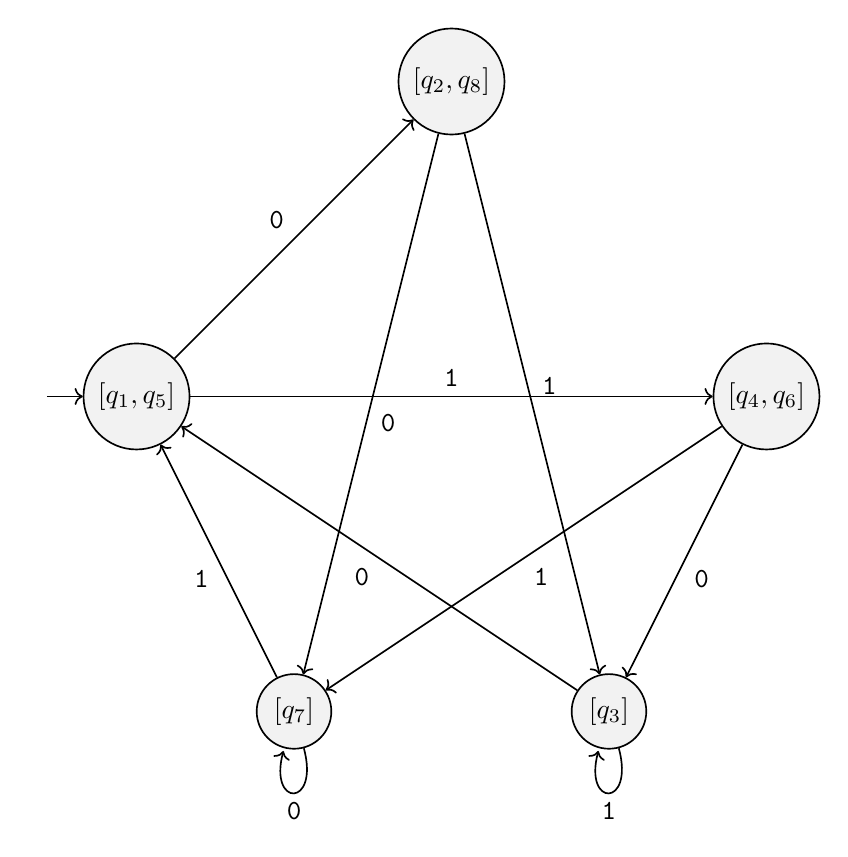
\begin{tikzpicture}
\node[state, initial] (A) at (0,0) {$[q_{1} , q_{5}]$};
\node[state] (B) at (4,4) {$[q_{2}, q_{8}]$};
\node[state] (C) at (8,0) {$[q_{4}, q_{6}]$};
\node[state] (D) at (2,-4) {$[q_{7}]$};
\node[state] (E) at (6,-4) {$[q_{3}]$};
\draw (A) edge node{\tt 0} (B);
\draw (A) edge node{\tt 1} (C);
\draw (B) edge node{\tt 0} (D);
\draw (B) edge node{\tt 1} (E);
\draw (C) edge node{\tt 0} (E);
\draw (C) edge node{\tt 1} (D);
\draw (D) edge node{\tt 1} (A);
\draw (D) edge[loop below] node{\tt 0} (D);
\draw (E) edge node{\tt 0} (A);
\draw (E) edge[loop below] node{\tt 1} (E);
\end{tikzpicture}

\section{Definition of a Grammar}

a Grammar is $(V , \Sigma , S , P)$, where :

\begin{itemize}
	\item $V$ is a finite non-empty set whose elements are variables
	\item $\Sigma$ or $T$ is a finite non-empty set whose elements are terminals
	$$
	V \cap \Sigma = \phi
	$$
	\item $S$ is a start symbol, where $S \in V$
	\item $P$ is a finite set whose elements are $\alpha \to \beta$, known as production rules, where, $\alpha, \beta \in ( V \cup \Sigma )^{*}$ , $\alpha$ should contain at least one symbol from $V$.
\end{itemize}

\subsection{Example}

$G = (V , \Sigma, S , P) $ is a grammar where :


\begin{align*}
V &= \{ <sentence> , <noun> , <adj> , <verb> , <art> \} \\
\Sigma &= \{ Ram, Rita, Azad, is , are, a , an , good, bad , boy , girl \} \\
S &= <sentence> \\
\end{align*}


$P$ consists of the following production rules :

\begin{align*}
<sentence> &\to <noun><verb><art><adj><noun> \\
<noun> &\to Ram | Rita | Azad | boy | girl \\
<verb> &\to is | are \\
<art> &\to a | an \\
<adj> &\to good | bad  \\
\end{align*}


An Example Parse Tree For this Grammar is :

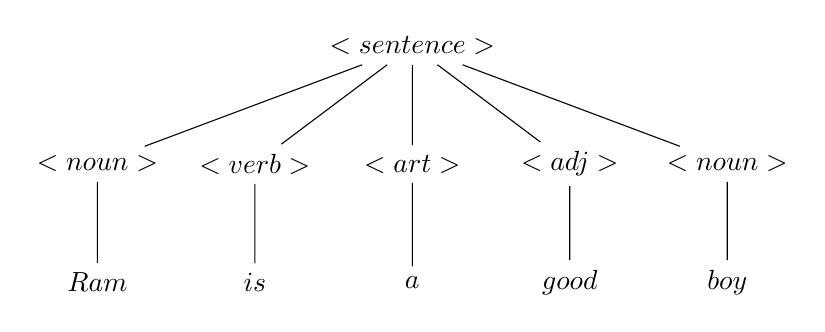
\begin{tikzpicture}[sibling distance=2cm]
\node {$<sentence>$}
child {node {$<noun>$}
	child {node {$Ram$}}
}
child {node {$<verb>$}
	child {node {$is$}}
}
child {node {$<art>$}
	child {node {$a$}}
}
child {node {$<adj>$}
	child {node {$good$}}
}
child {node {$<noun>$}
	child {node {$boy$}}
};
\end{tikzpicture}



\subsection{Example}

Determine the Grammer G Where :

$$
L(G) = \{ 0^{n} 1 ^{n} | n \geq 0 \}
$$

Answer :

$ S \to 0S1 | \lambda $

sample : $0^{3} 1 ^{3}$

$S \to 0S1 \to 00S11 \to 000S111 \to 000111 \equiv 0^{3} 1 ^{3}$

\begin{align*}
G &= (V, \Sigma, S, P) \\
V &= \{ S \} \\
\Sigma &= \{ 0, 1 \} \\
S &= S \\
P &= \{ S \to 0S1 , S \to \lambda \}  \\
\end{align*}


\subsection{Example}

Determine the Grammar G Where :

$$
L(G) = \{ 0^{n} 1 ^{n} | n \geq 1 \}
$$

Answer :

$ S \to 0S1 | 01 $


\begin{align*}
G &= (V, \Sigma, S, P) \\
V &= \{ S \} \\
\Sigma &= \{ 0, 1 \} \\
S &= S \\
P &= \{ S \to 0S1 , S \to 01 \}  \\
\end{align*}


\subsection{Example}

Determine the Grammar G Where :

$$
L(G) = \{ a^{n} b ^{m} c ^{k} | n , k > 0 \: and \: m \geq 0 \}
$$

Answer :

\begin{align*}
 S &\to S_{1}S_{2}S_{3} \\
 S_{1} &\to aS_{1} | a  \\
 S_{2} &\to bS_{2} | \lambda  \\
 S_{3} &\to cS_{3} | c \\
\end{align*}

\begin{align*}
G &= (V, \Sigma, S, P) \\
V &= \{ S , S_{1} , S_{2} , S_{3} \} \\
\Sigma &= \{ a, b, c \} \\
S &= S \\
P &= \{ S \to S_{1}S_{2}S_{3} ,
S_{1} \to aS_{1} | a ,
S_{2} \to bS_{2} | \lambda ,
S_{3} \to cS_{3} | c  \}  \\
\end{align*}

\subsection{Example}

Determine the Grammar G Where :

$$
L(G) = \{ a^{n} b ^{m} c ^{k} | n \geq 0 \: , k > 1 \:, m = n + k \}
$$

Answer :

\begin{align*}
 S &\to S_{1}S_{2} \\
 S_{1} &\to aS_{1}b | \lambda  \\
 S_{2} &\to bS_{2}c | bbcc  \\
\end{align*}


\begin{align*}
G &= (V, \Sigma, S, P) \\
V &= \{ S , S_{1} , S_{2} \} \\
\Sigma &= \{ a, b, c \} \\
S &= S \\
P &= \{ S \to S_{1}S_{2} ,
S_{1} \to aS_{1}b | \lambda ,
S_{2} \to bS_{2}c | bbcc \}
\end{align*}


\subsection{Example}


Determine the Grammar G Where :

$$
L(G) = \{ a^{n} b ^{m} | n > m \geq 1 \}
$$

Answer :

\begin{align*}
 S &\to aS | aSb | aab \\
\end{align*}


\begin{align*}
G &= (V, \Sigma, S, P) \\
V &= \{ S \} \\
\Sigma &= \{ a, b\} \\
S &= S \\
P &= \{ S \to aS ,
S \to aSb  ,
S \to aab  \}
\end{align*}


\subsection{Example}

Determine the Grammar G Where :

$$
L(G) = \{ (ab)^{n} c ^{n} | n \geq 1 \}
$$

Answer :

\begin{align*}
 S &\to abSc | abc \\
\end{align*}


\begin{align*}
G &= (V, \Sigma, S, P) \\
V &= \{ S \} \\
\Sigma &= \{ a, b, c \} \\
S &= S \\
P &= \{ S \to abSc ,
S \to abc  \}
\end{align*}


\subsection{Example}

Determine the Grammar G Where :

$$
L(G) = \{ (x)^{2n} y ^{n} | n \geq 1 \}
$$

Answer :

\begin{align*}
 S &\to xxSy | xxy \\
\end{align*}


\begin{align*}
G &= (V, \Sigma, S, P) \\
V &= \{ S \} \\
\Sigma &= \{ x, y \} \\
S &= S \\
P &= \{ S \to xxSy ,
S \to xxy  \}
\end{align*}



\subsection{Example}

Determine the Grammar G Where :

$$
L(G) = \{ \omega c \omega^{T} | \omega \in (a,b)^{*} \}
$$

Sample : 
$$
\underbrace{abb}_{\omega}c\underbrace{bba}_{\omega^{T}}
$$

Answer :

\begin{align*}
 S &\to aSa | bSb | c \\
\end{align*}


\begin{align*}
G &= (V, \Sigma, S, P) \\
V &= \{ S \} \\
\Sigma &= \{ x, y \} \\
S &= S \\
P &= \{ S \to aSa ,
S \to bSb ,
S \to c  \}
\end{align*}


\subsection{Example}


Determine the Grammar G Where :

$$
L(G) = \{ \omega c \omega^{T} | \omega \in (a,b)^{+} \}
$$

Answer :

\begin{align*}
 S &\to aSa | bSb | aca | bcb \\
\end{align*}


\begin{align*}
G &= (V, \Sigma, S, P) \\
V &= \{ S \} \\
\Sigma &= \{ a, b, c \} \\
S &= S \\
P &= \{ S \to aSa ,
S \to bSb ,
S \to aca , 
S \to bcb \}
\end{align*}



\subsection{Example}

Determine the Grammar G Where :

$$
L(G) = \{ a^{n} b^{m} | \:where\: n\: is\: even\: and\: m\: is\: odd\: \}
$$

Answer :

\begin{align*}
 S &\to S_{1}S_{2} \\
 S_{1} &\to aaS_{1} | \wedge \\
 S_{2} &\to bbS_{2} | b \\
\end{align*}

note : one extra b cause odd number of b

\begin{align*}
G &= (V, \Sigma, S, P) \\
V &= \{ S , S_{1} , S_{2} \} \\
\Sigma &= \{ a, b \} \\
S &= S \\
P &= \{ S \to S_{1}S_{2}b ,
S_{1} \to aaS_{1} | \wedge ,
S_{1} \to bbS_{2} | b \}
\end{align*}


\subsection{Example}

Determine the Grammar G Where :

$$
L(G) = \{ a^{n} b^{m} c^{m} d^{n}  | n \geq 1 , m \geq 0 \}
$$

Answer :

\begin{align*}
 S &\to aSd | aS_{1}d \\
 S_{1} &\to bS_{1}c | \wedge \\
\end{align*}


\begin{align*}
G &= (V, \Sigma, S, P) \\
V &= \{ S , S_{1} \} \\
\Sigma &= \{ a, b, c, d \} \\
S &= S \\
P &= \{ S \to aSd ,
S_{1} \to aSd | aS_{1}d ,
S_{1} \to bS_{1}c | \wedge , 
S \to bcb \}
\end{align*}


\subsection{Example}

Determine the Grammar G Where :

$$
L(G) = \{ a^{n} b^{n} c^{n}  | n \geq 1 \}
$$

Answer :

if n = 3 then $\omega = aaabbbccc \equiv a^{3} b^{3} c^{3}$ .

let us apply $S \to aSBC$ for $(n-1)$ number of times .

\begin{align*}
 S &\to aSBC \\
  &\to aaSBCBC \\
\end{align*}

now apply $S \to aBC$ once :

\begin{align*}
  &\to aaaBCBCBC \\
\end{align*}

now apply $CB \to BC$ :

\begin{align*}
  &\to aaaB\underbrace{CB}_{BC}\underbrace{CB}_{BC}C \\
  &\to aaaBB\underbrace{CB}_{BC}CC \\
  &\to aaaBBBCCC
\end{align*}

we shall apply $aB \to ab$ :

\begin{align*}
  &\to aa\underbrace{aB}_{ab}BBCCC \\
  &\to aaabBBCCC \\
\end{align*}

Now we apply $bB \to bb$ :

\begin{align*}
  &\to aaa\underbrace{bB}_{ab}BCCC \\
  &\to aaab\underbrace{bB}_{bb}CCC \\
  &\to aaabbbCCC \\
\end{align*}

Now we apply $bC \to bc$ :

\begin{align*}
  &\to aaabb\underbrace{bC}_{bc}CC \\
  &\to aaabbbcCC \\
\end{align*}


Now we apply $cC \to cc$ :

\begin{align*}
  &\to aaabbb\underbrace{cC}_{cc}C \\
  &\to aaabbbc\underbrace{cC}_{cc} \\
  &\to aaabbbccc
\end{align*}



\begin{align*}
G &= (V, \Sigma, S, P) \\
V &= \{ S , B, C \} \\
\Sigma &= \{ a, b, c \} \\
S &= S \\
P &= \{ S \to aSBC ,
S \to aBC ,
CB \to BC ,
aB \to ab ,
bB \to bb ,
bC \to bc ,
cC \to cc \}
\end{align*}


\subsection{Example}

Find the language generated the following Grammar :

\begin{align*}
S &\to 0S1 \\
S &\to 0A1 \\
A &\to 1A \\
A &\to 1 \\
\end{align*}


answer :

$$
L(G) = \{ 0^{m}1^{n} | n > m \geq 1 \}
$$


\chapter{Regular Expressions and Identities}

we are mainly concerned with the characterization of sets of strings recognized by finite automata .
It is therefore appropriate to develope a compact language for describing such sets of strings, the language thus developed is known as type-3 language or as the language of regular expressions .
some sample string are 101, (01+10)11 , $\dots$

note : 

$$
1^{*} = \lambda + 1 + 11 + 111 + 1111 + \dots
$$

$$
1^{+} = 1 + 11 + 111 + 1111 + \dots
$$

$$
\Rightarrow 1^{*} = 1^{+} \cup \lambda
$$

\section{Identities of Regular Expressions}

\begin{align*}
I_{1} &: \phi + R = R \\
I_{2} &: \phi R + R \phi = \phi \\
I_{3} &: \wedge R + R \wedge = R \\
I_{4} &: \wedge^{*}  = \wedge \:\: and \:\: \phi^{*} = \wedge \\
I_{5} &: R + R = R \\
I_{6} &: R^{*} R^{*} = R^{*} \\
I_{7} &: R R^{*} = R^{*} R = R^{+} \\
I_{8} &: (R^{*})^{*} = R^{*} \\
I_{9} &: \wedge + R R^{*} = R^{*} = \wedge +  R^{*} R \\
I_{10} &: (PQ)^{*} P = P (QP)^{*} \\
I_{11} &: (P + Q)^{*} = (P^{*} Q^{*})^{*} = (P^{*} + Q^{*})^{*} \\
I_{12} &: (P + Q) R = P R + Q R \\
&and \\
&: R (P + Q) = R P + R Q
\end{align*}


\section{difference between $\wedge$ and $\phi$}

you can't reach to final state when $R = \phi$ but when $R = \wedge$ you can reach at final state with empty input .


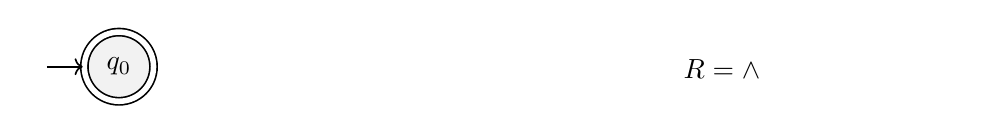
\begin{tikzpicture}
\node[state, initial, accepting] (q0) at (0,0) {$q_{0}$};
\draw[shift={(60:1cm)},xshift=4cm,yshift=-.8cm]
node [right,text width=6cm,rounded corners,fill=white,inner sep=1ex]
{
$$ 
R = \wedge
$$
};
\end{tikzpicture}


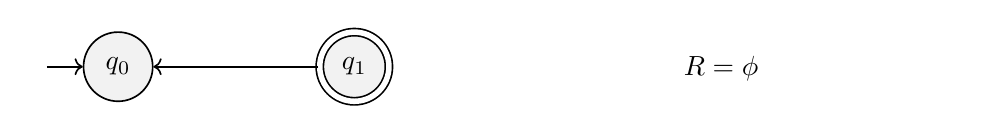
\begin{tikzpicture}
\node[state, initial] (q0) at (0,0) {$q_{0}$};
\node[state, accepting] (q1) at (3,0) {$q_{1}$};
\draw (q1) edge node{} (q0);
\draw[shift={(60:1cm)},xshift=4cm,yshift=-.8cm]
node [right,text width=6cm,rounded corners,fill=white,inner sep=1ex]
{
$$ 
R = \phi
$$
};
\end{tikzpicture}


\section{Regular Expressions and Transition Systems}

\begin{enumerate}
	\item $(R_{1} + R_{2})$ :
	
	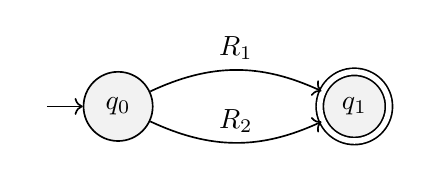
\begin{tikzpicture}
	\node[state, initial] (q0) at (0,0) {$q_{0}$};
	\node[state, accepting] (q1) at (3,0) {$q_{1}$};
	\draw (q0) edge[bend left=25] node{$R_{1}$} (q1);
	\draw (q0) edge[bend right=25] node{$R_{2}$} (q1);
	\end{tikzpicture}
	
	\item $(R_{1} R_{2})$ :
	
	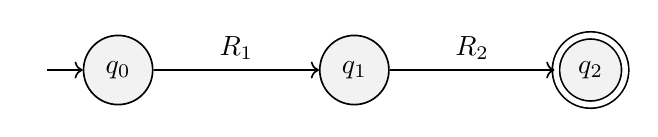
\begin{tikzpicture}
	\node[state, initial] (q0) at (0,0) {$q_{0}$};
	\node[state] (q1) at (3,0) {$q_{1}$};
	\node[state, accepting] (q2) at (6,0) {$q_{2}$};
	\draw (q0) edge node{$R_{1}$} (q1);
	\draw (q1) edge node{$R_{2}$} (q2);
	\end{tikzpicture}
	
	\item $(R_{1} + R_{2})^{*}$ :
	
	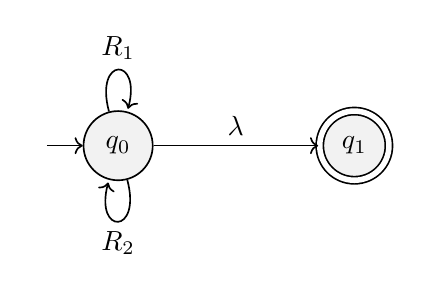
\begin{tikzpicture}
	\node[state, initial] (q0) at (0,0) {$q_{0}$};
	\node[state, accepting] (q1) at (3,0) {$q_{1}$};
	\draw (q0) edge[loop above] node{$R_{1}$} (q0);
	\draw (q0) edge[loop below] node{$R_{2}$} (q0);
	\draw (q0) edge node{$\lambda$} (q1);
	\end{tikzpicture}
	
	$$OR$$
	
	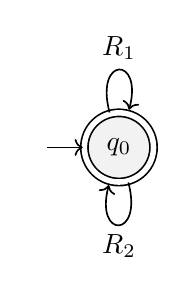
\begin{tikzpicture}
	\node[state, initial, accepting] (q0) at (0,0) {$q_{0}$};
	\draw (q0) edge[loop above] node{$R_{1}$} (q0);
	\draw (q0) edge[loop below] node{$R_{2}$} (q0);
	\end{tikzpicture}
	
	\item $(R_{1} + R_{2})^{+}$ :
	
	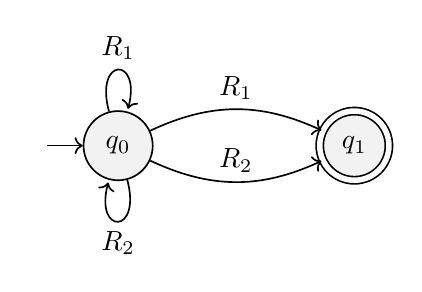
\begin{tikzpicture}
	\node[state, initial] (q0) at (0,0) {$q_{0}$};
	\node[state, accepting] (q1) at (3,0) {$q_{1}$};
	\draw (q0) edge[loop above] node{$R_{1}$} (q0);
	\draw (q0) edge[loop below] node{$R_{2}$} (q0);
	\draw (q0) edge[bend left=25] node{$R_{1}$} (q1);
	\draw (q0) edge[bend right=25] node{$R_{2}$} (q1);
	\end{tikzpicture}
	
	
	\item $(R_{1} R_{2})^{*}$ :
	
	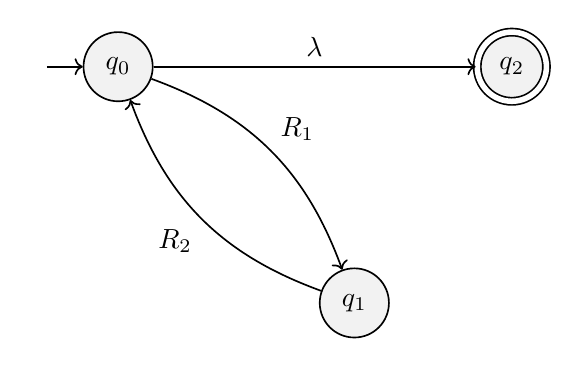
\begin{tikzpicture}
	\node[state, initial] (q0) at (0,0) {$q_{0}$};
	\node[state] (q1) at (3,-3) {$q_{1}$};
	\node[state, accepting] (q2) at (5,0) {$q_{2}$};
	\draw (q0) edge[bend left=25] node{$R_{1}$} (q1);
	\draw (q1) edge[bend left=25] node{$R_{2}$} (q0);
	\draw (q0) edge node{$\lambda$} (q2);
	\end{tikzpicture}
	
	
	\item $(R_{1} R_{2})^{+}$ :
	
	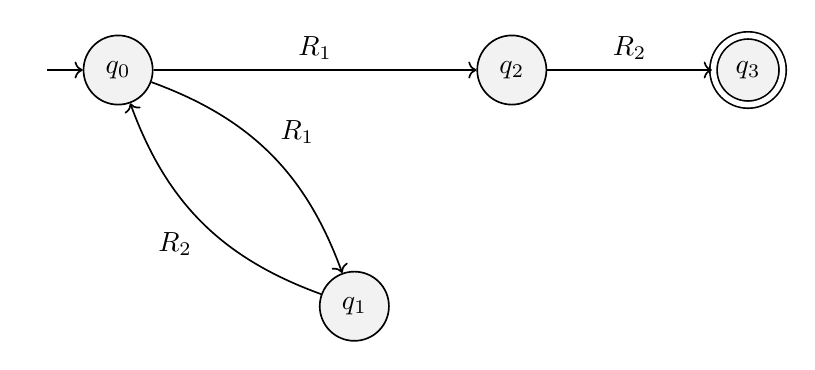
\begin{tikzpicture}
	\node[state, initial] (q0) at (0,0) {$q_{0}$};
	\node[state] (q1) at (3,-3) {$q_{1}$};
	\node[state] (q2) at (5,0) {$q_{2}$};
	\node[state, accepting] (q3) at (8,0) {$q_{3}$};
	\draw (q0) edge[bend left=25] node{$R_{1}$} (q1);
	\draw (q1) edge[bend left=25] node{$R_{2}$} (q0);
	\draw (q0) edge node{$R_{1}$} (q2);
	\draw (q2) edge node{$R_{2}$} (q3);
	\end{tikzpicture}
	
	
	\item $R_{1}^{*}(R_{2} + R_{3})R_{4}^{*}$ :
	
	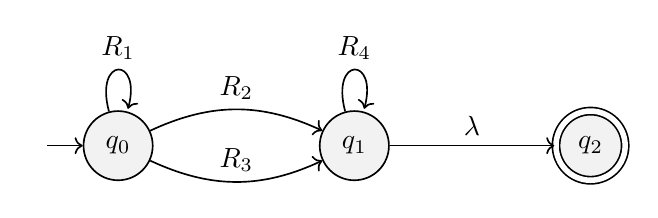
\begin{tikzpicture}
	\node[state, initial] (q0) at (0,0) {$q_{0}$};
	\node[state] (q1) at (3,0) {$q_{1}$};
	\node[state, accepting] (q2) at (6,0) {$q_{2}$};
	\draw (q0) edge[loop above] node{$R_{1}$} (q0);
	\draw (q0) edge[bend left=25] node{$R_{2}$} (q1);
	\draw (q0) edge[bend right=25] node{$R_{3}$} (q1);
	\draw (q1) edge[loop above] node{$R_{4}$} (q1);
	\draw (q1) edge node{$\lambda$} (q2);
	\end{tikzpicture}
	
	
	
	\item $R_{1}(R_{2}^{*} + R_{3}^{*})R_{4}$ :
	
	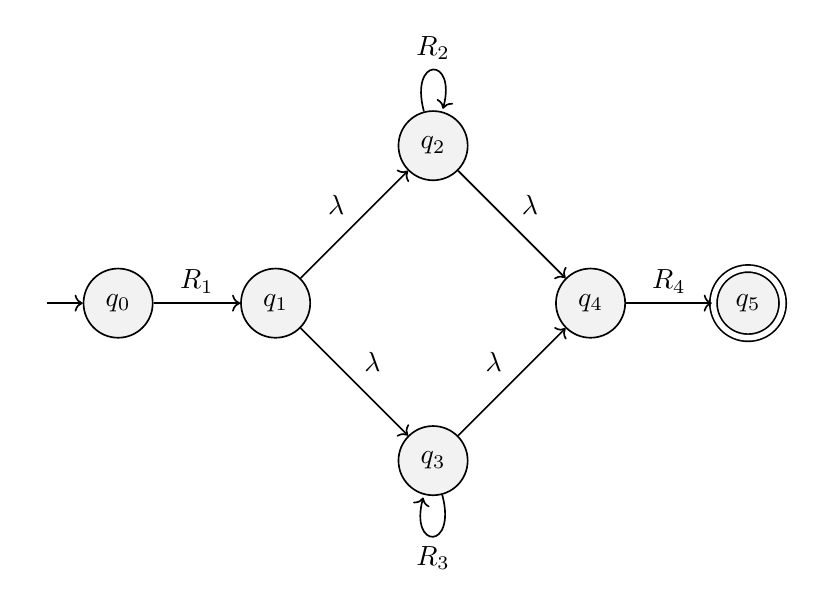
\begin{tikzpicture}
	\node[state, initial] (q0) at (0,0) {$q_{0}$};
	\node[state] (q1) at (2,0) {$q_{1}$};
	\node[state] (q2) at (4,2) {$q_{2}$};
	\node[state] (q3) at (4,-2) {$q_{3}$};
	\node[state] (q4) at (6,0) {$q_{4}$};
	\node[state, accepting] (q5) at (8,0) {$q_{5}$};
	\draw (q0) edge node{$R_{1}$} (q1);
	\draw (q1) edge node{$\lambda$} (q2);
	\draw (q1) edge node{$\lambda$} (q3);
	\draw (q2) edge node{$\lambda$} (q4);
	\draw (q2) edge[loop above] node{$R_{2}$} (q2);
	\draw (q3) edge node{$\lambda$} (q4);
	\draw (q3) edge[loop below] node{$R_{3}$} (q3);
	\draw (q4) edge node{$R_{4}$} (q5);
	\end{tikzpicture}
	
	
	
	\item $R_{1}R_{2}^{*}R_{3} + R_{4}R_{5}^{*}R_{6}$ :
	
	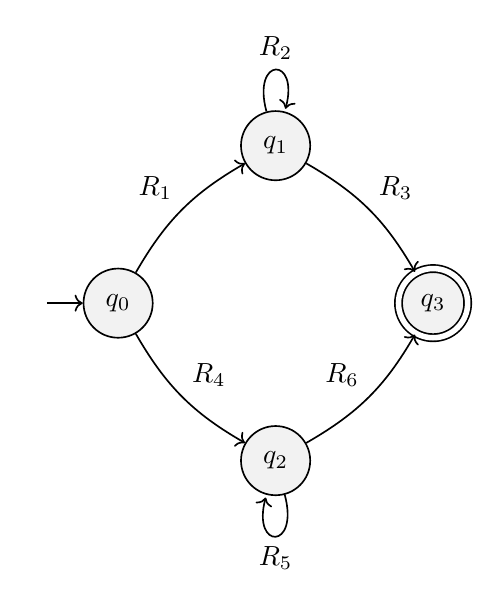
\begin{tikzpicture}
	\node[state, initial] (q0) at (0,0) {$q_{0}$};
	\node[state] (q1) at (2,2) {$q_{1}$};
	\node[state] (q2) at (2,-2) {$q_{2}$};
	\node[state , accepting] (q3) at (4,0) {$q_{3}$};
	\draw (q0) edge[bend left=15] node{$R_{1}$} (q1);
	\draw (q0) edge[bend right=15] node{$R_{4}$} (q2);
	\draw (q1) edge[loop above] node{$R_{2}$} (q1);
	\draw (q1) edge[bend left=15] node{$R_{3}$} (q3);
	\draw (q2) edge[loop below] node{$R_{5}$} (q2);
	\draw (q2) edge[bend right=15] node{$R_{6}$} (q3);
	\end{tikzpicture}
	
	
	
	\item $(R_{1} + R_{2}) (R_{3} + R_{4})$ :
	
	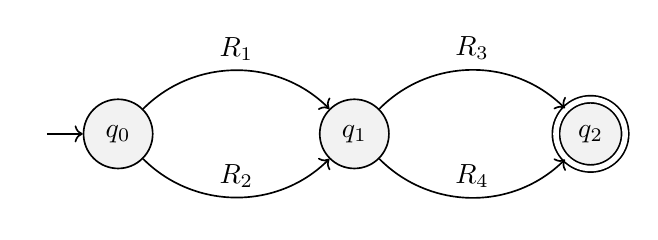
\begin{tikzpicture}
	\node[state, initial] (q0) at (0,0) {$q_{0}$};
	\node[state] (q1) at (3,0) {$q_{1}$};
	\node[state, accepting] (q2) at (6,0) {$q_{2}$};
	\draw (q0) edge[bend left=45] node{$R_{1}$} (q1);
	\draw (q0) edge[bend right=45] node{$R_{2}$} (q1);
	\draw (q1) edge[bend left=45] node{$R_{3}$} (q2);
	\draw (q1) edge[bend right=45] node{$R_{4}$} (q2);
	\end{tikzpicture}
	
	
	\item $R_{1}^{*} R_{2} R_{3}^{*} +R_{4}^{*} R_{5} R_{6}^{*}$ :
	
	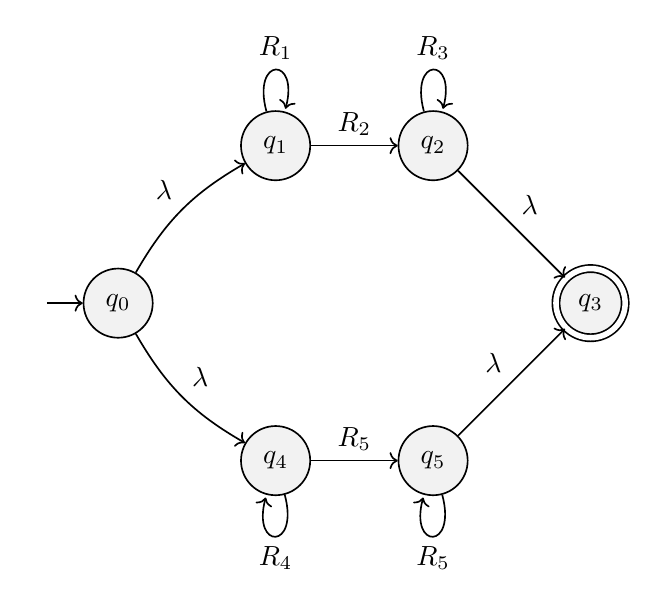
\begin{tikzpicture}
	\node[state, initial] (q0) at (0,0) {$q_{0}$};
	\node[state] (q1) at (2,2) {$q_{1}$};
	\node[state] (q2) at (4,2) {$q_{2}$};
	\node[state, accepting] (q3) at (6,0) {$q_{3}$};
	\node[state] (q4) at (2,-2) {$q_{4}$};
	\node[state] (q5) at (4,-2) {$q_{5}$};
	\draw (q0) edge[bend left=15] node{$\lambda$} (q1);
	\draw (q1) edge[loop above] node{$R_{1}$} (q1);
	\draw (q1) edge node{$R_{2}$} (q2);
	\draw (q2) edge[loop above] node{$R_{3}$} (q2);
	\draw (q2) edge node{$\lambda$} (q3);
	\draw (q0) edge[bend right=15] node{$\lambda$} (q4);
	\draw (q4) edge[loop below] node{$R_{4}$} (q4);
	\draw (q4) edge node{$R_{5}$} (q5);
	\draw (q5) edge node{$\lambda$} (q3);
	\draw (q5) edge[loop below] node{$R_{5}$} (q5);
	\end{tikzpicture}
	
	
	\item $R_{1}^{*} (R_{1} R_{2})^{+}$ :
	
	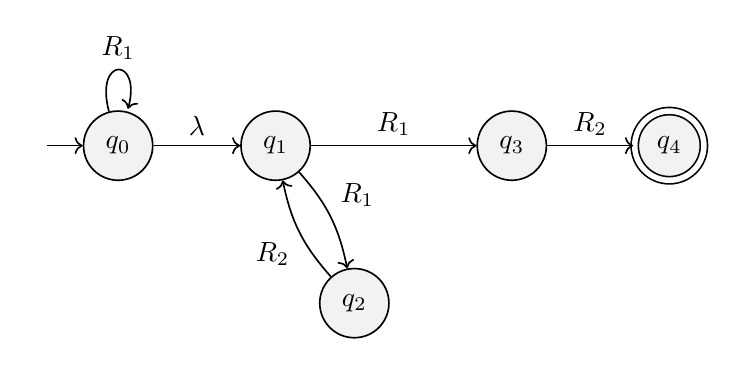
\begin{tikzpicture}
	\node[state, initial] (q0) at (0,0) {$q_{0}$};
	\node[state] (q1) at (2,0) {$q_{1}$};
	\node[state] (q2) at (3,-2) {$q_{2}$};
	\node[state] (q3) at (5,0) {$q_{3}$};
	\node[state , accepting] (q4) at (7,0) {$q_{4}$};
	\draw (q0) edge[loop above] node{$R_{1}$} (q0);
	\draw (q0) edge node{$\lambda$} (q1);
	\draw (q1) edge[bend left=15] node{$R_{1}$} (q2);
	\draw (q2) edge[bend left=15] node{$R_{2}$} (q1);
	\draw (q1) edge node{$R_{1}$} (q3);
	\draw (q3) edge node{$R_{2}$} (q4);
	\end{tikzpicture}
	
\end{enumerate}


\section{$\lambda$ transition elimination }

\textbf{Rules : }

\begin{itemize}
	\item Find all the edges starting from $V_{2}$
	\item Duplicate all these edges starting from $V_{1}$ , without changing the edge labels
	\item If $V_{1}$ is the initial state, make $V_{2}$ also initial state
	\item If $V_{2}$ is the final state, make $V_{1}$ as final state
\end{itemize}

\subsection{Example}

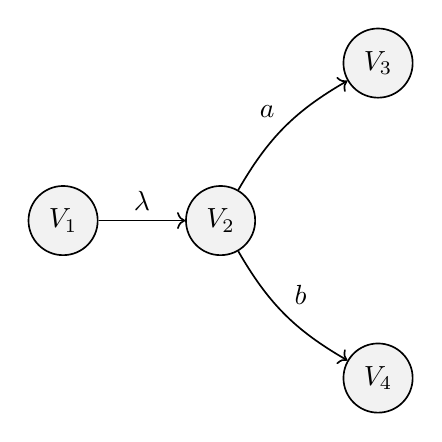
\begin{tikzpicture}
\node[state] (v1) at (0,0) {$V_{1}$};
\node[state] (v2) at (2,0) {$V_{2}$};
\node[state] (v3) at (4,2) {$V_{3}$};
\node[state] (v4) at (4,-2) {$V_{4}$};
\draw (v1) edge node{$\lambda$} (v2);
\draw (v2) edge[bend left=15] node{$a$} (v3);
\draw (v2) edge[bend right=15] node{$b$} (v4);
\end{tikzpicture}

After removing $\lambda$ transition :

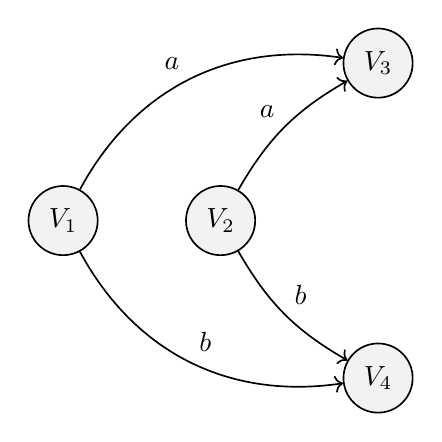
\begin{tikzpicture}
\node[state] (v1) at (0,0) {$V_{1}$};
\node[state] (v2) at (2,0) {$V_{2}$};
\node[state] (v3) at (4,2) {$V_{3}$};
\node[state] (v4) at (4,-2) {$V_{4}$};
\draw (v1) edge[bend left=35] node{$a$} (v3);
\draw (v1) edge[bend right=35] node{$b$} (v4);
\draw (v2) edge[bend left=15] node{$a$} (v3);
\draw (v2) edge[bend right=15] node{$b$} (v4);
\end{tikzpicture}


\subsection{Example}

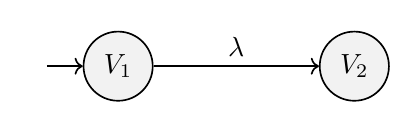
\begin{tikzpicture}
\node[state, initial] (v1) at (0,0) {$V_{1}$};
\node[state] (v2) at (3,0) {$V_{2}$};
\draw (v1) edge node{$\lambda$} (v2);
\end{tikzpicture}

after :

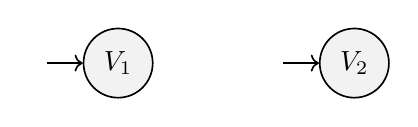
\begin{tikzpicture}
\node[state, initial] (v1) at (0,0) {$V_{1}$};
\node[state, initial] (v2) at (3,0) {$V_{2}$};
\end{tikzpicture}


\subsection{Example}

eliminate the $\lambda$ transition :

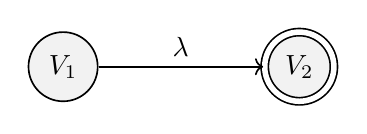
\begin{tikzpicture}
\node[state] (v1) at (0,0) {$V_{1}$};
\node[state, accepting] (v2) at (3,0) {$V_{2}$};
\draw (v1) edge node{$\lambda$} (v2);
\end{tikzpicture}

after :

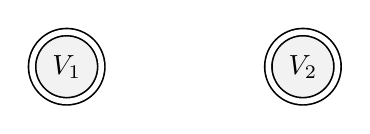
\begin{tikzpicture}
\node[state, accepting] (v1) at (0,0) {$V_{1}$};
\node[state, accepting] (v2) at (3,0) {$V_{2}$};
\end{tikzpicture}


\subsection{Example}

eliminate the $\lambda$ transition :

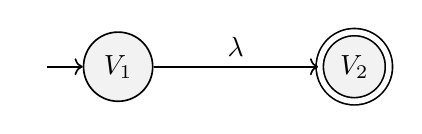
\begin{tikzpicture}
\node[state, initial] (v1) at (0,0) {$V_{1}$};
\node[state, accepting] (v2) at (3,0) {$V_{2}$};
\draw (v1) edge node{$\lambda$} (v2);
\end{tikzpicture}

after :

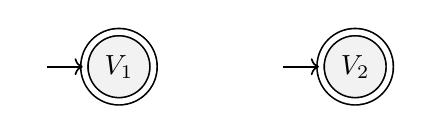
\begin{tikzpicture}
\node[state,  initial, accepting] (v1) at (0,0) {$V_{1}$};
\node[state,  initial, accepting] (v2) at (3,0) {$V_{2}$};
\end{tikzpicture}


\subsection{Example}

Simple the Regular expressions below :

\begin{align*}
 & 10 + (1010)^{*} [ \lambda^{*} + \underbrace{\lambda(1010)^{*}}_{(1010)^{*}} ]  \\
 &\to 10 + (1010)^{*} [ \underbrace{\lambda^{*} + (1010)^{*}}_{(1010)^{*}} ] \\
 &\to 10 + \underbrace{(1010)^{*} (1010)^{*}}_{(1010)^{*}} \\
 &\to 10 + (1010)^{*} \\
\end{align*}


\subsection{Example}

Consider the following transition system 

	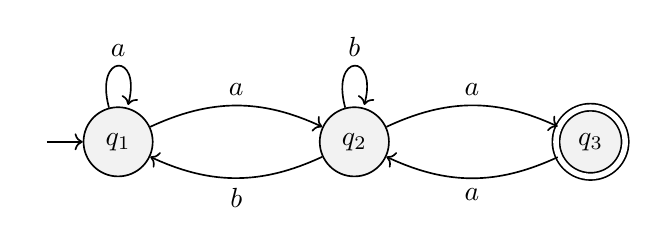
\begin{tikzpicture}
	\node[state, initial] (q0) at (0,0) {$q_{1}$};
	\node[state] (q1) at (3,0) {$q_{2}$};
	\node[state, accepting] (q2) at (6,0) {$q_{3}$};
	\draw (q0) edge[bend left=25] node{$a$} (q1);
	\draw (q0) edge[loop above] node{$a$} (q0);
	\draw (q1) edge[bend left=25] node{$b$} (q0);
	\draw (q1) edge[loop above] node{$b$} (q1);
	\draw (q1) edge[bend left=25] node{$a$} (q2);
	\draw (q2) edge[bend left=25] node{$a$} (q1);
	\end{tikzpicture}


Find out which regular expressions can be deducted from this transition system :


\begin{align}
q_{1} &= q_{1}a + q_{2}b + \wedge \\
q_{2} &= q_{1}a + q_{2}b + q_{3}a \\
q_{3} &= q_{2}a 
\end{align}

using (2.1) and (2.2) we have :


\begin{align*}
q_{2} &= q_{1}a + q_{2}b + q_{2}aa \\
 &= \underbrace{q_{1}a}_{Q} + \underbrace{q_{2}}_{R}\underbrace{(b + aa)}_{P} \\
\end{align*}

Arden's Theorem :
$$
R = Q + RP \to R = QP^{*}
$$

and we have :

\begin{align*}
q_{2} &= q_{1}a (b + aa)^{*} \\
\end{align*}


\begin{align*}
\underbrace{q_{1}}_{R} &= q_{1}a + q_{1}a(b + aa)^{*} b + \wedge \\
&= \underbrace{q_{1}}_{R} \underbrace{(a + a(b+aa)^{*}b)}_{P} + \underbrace{\wedge}_{Q}
\end{align*}

According to Arden's Theorem :

\begin{align*}
q_{1} &=  \wedge (a + a(b+aa)^{*}b)^{*} \\
&=  (a + a(b+aa)^{*}b)^{*} 
\end{align*}


\begin{align*}
q_{2} &=  q_{1}a(b + aa)^{*} \\
&= (a + a(b + aa)^{*}b)^{*}a(b + aa)^{*}
\end{align*}


\begin{align*}
q_{3} &=  q_{2}a \\
&= (a + a(b + aa)^{*}b)^{*}a(b + aa)^{*}a
\end{align*}



\section{Arden's Theorem}

Let P and Q be two regular expressions over $\Sigma$ if P does not contain $\wedge$, then the following equation in R :
$$
R = Q + R P
$$
has unique solution (one and only one) :
$$
R = Q P^{*}
$$

Proof :
put $R =  QP^{*}$ in the $R = Q + R P$ formula

\begin{align*}
QP^{*} &= Q + (QP^{*})P \\
&= Q (\wedge + \underbrace{P^{*}P}_{P^{*}} ) \\
&= Q( \underbrace{\wedge + P^{*}}_{P^{*}})
&= QP^{*}
\end{align*}


\subsection{Example}

Construct a Finite Automata equivalent to the regular expressoin :

$$
(0 + 1)^{*} (00 + 11) (0 + 1)^{*}
$$

Suppose :

$$
R_{1}^{*} R_{2} R_{3}^{*}
$$

$$
R_{1}^{*} (R_{21} + R_{22}) R_{3}^{*}
$$

now we can have :

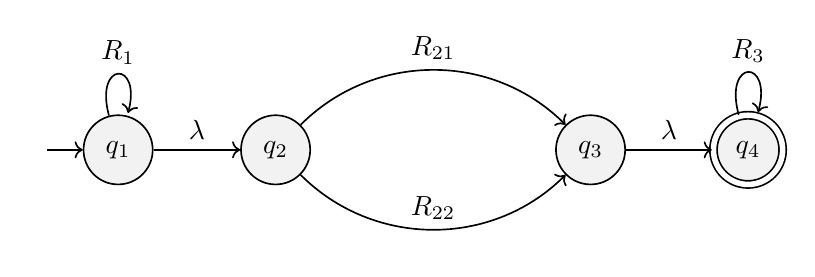
\begin{tikzpicture}
\node[state, initial] (q0) at (0,0) {$q_{1}$};
\node[state] (q1) at (2,0) {$q_{2}$};
\node[state] (q2) at (6,0) {$q_{3}$};
\node[state, accepting] (q3) at (8,0) {$q_{4}$};
\draw (q0) edge node{$\lambda$} (q1);
\draw (q0) edge[loop above] node{$R_{1}$} (q0);
\draw (q1) edge[bend left=45] node{$R_{21}$} (q2);
\draw (q1) edge[bend right=45] node{$R_{22}$} (q2);
\draw (q2) edge node{$\lambda$} (q3);
\draw (q3) edge[loop above] node{$R_{3}$} (q3);
\end{tikzpicture}

then we can design :


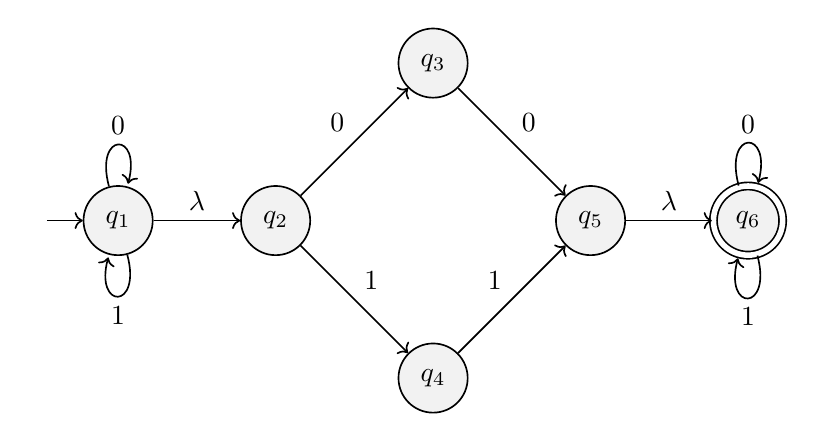
\begin{tikzpicture}
\node[state, initial] (q0) at (0,0) {$q_{1}$};
\node[state] (q1) at (2,0) {$q_{2}$};
\node[state] (q2) at (4,2) {$q_{3}$};
\node[state] (q3) at (4,-2) {$q_{4}$};
\node[state] (q4) at (6,0) {$q_{5}$};
\node[state , accepting] (q5) at (8,0) {$q_{6}$};
\draw (q0) edge node{$\lambda$} (q1);
\draw (q0) edge[loop above] node{$0$} (q0);
\draw (q0) edge[loop below] node{$1$} (q0);
\draw (q1) edge node{$0$} (q2);
\draw (q2) edge node{$0$} (q4);
\draw (q1) edge node{$1$} (q3);
\draw (q3) edge node{$1$} (q4);
\draw (q4) edge node{$\lambda$} (q5);
\draw (q5) edge[loop above] node{$0$} (q5);
\draw (q5) edge[loop below] node{$1$} (q5);
\end{tikzpicture}



\subsection{Example}

Construct a Finite Automata equivalent to the regular expressions :

$$
R = ( 1 (00)^{*} + 01^{*}0 )^{*}
$$

Suppose we have :

$$
(R_{1} + R_{2} )^{*}
$$

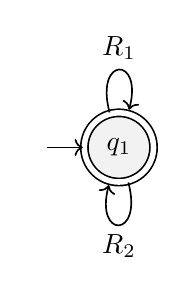
\begin{tikzpicture}
\node[state, initial, accepting] (q0) at (0,0) {$q_{1}$};
\draw (q0) edge[loop above] node{$R_{1}$} (q0);
\draw (q0) edge[loop below] node{$R_{2}$} (q0);
\end{tikzpicture}

so we have :

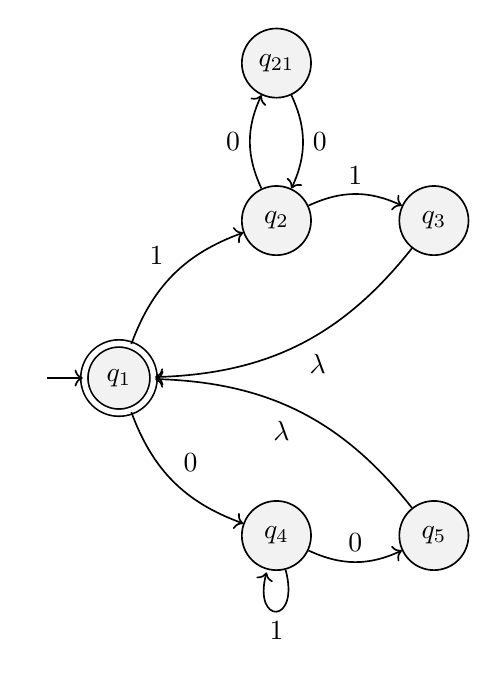
\begin{tikzpicture}
\node[state, initial, accepting] (q0) at (0,0) {$q_{1}$};
\node[state] (q1) at (2,2) {$q_{2}$};
\node[state] (q11) at (2,4) {$q_{21}$};
\node[state] (q2) at (4,2) {$q_{3}$};
\node[state] (q3) at (2,-2) {$q_{4}$};
\node[state] (q4) at (4,-2) {$q_{5}$};
\draw (q0) edge[bend left=25] node{$1$} (q1);
\draw (q1) edge[bend left=25] node{$1$} (q2);
\draw (q1) edge[bend left=25] node{$0$} (q11);
\draw (q11) edge[bend left=25] node{$0$} (q1);
\draw (q2) edge[bend left=25] node{$\lambda$} (q0);
\draw (q0) edge[bend right=25] node{$0$} (q3);
\draw (q3) edge[bend right=25] node{$0$} (q4);
\draw (q3) edge[loop below] node{$1$} (q3);
\draw (q4) edge[bend right=25] node{$\lambda$} (q0);
\end{tikzpicture}


if we want to do $\lambda-transition$ elimination we have :

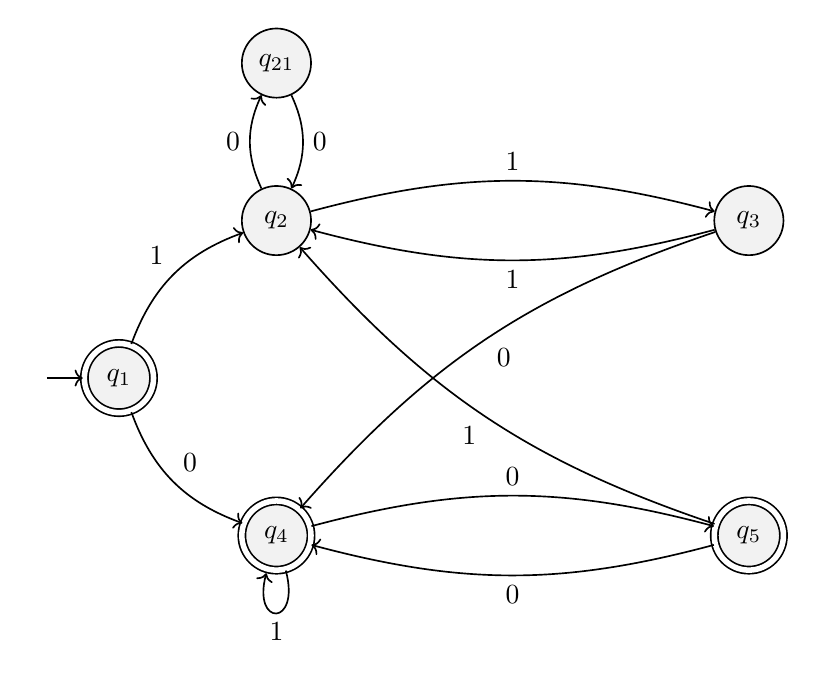
\begin{tikzpicture}
\node[state, initial, accepting] (q0) at (0,0) {$q_{1}$};
\node[state] (q1) at (2,2) {$q_{2}$};
\node[state] (q11) at (2,4) {$q_{21}$};
\node[state] (q2) at (8,2) {$q_{3}$};
\node[state , accepting] (q3) at (2,-2) {$q_{4}$};
\node[state, accepting] (q4) at (8,-2) {$q_{5}$};
\draw (q0) edge[bend left=25] node{$1$} (q1);
\draw (q1) edge[bend left=15] node{$1$} (q2);
\draw (q1) edge[bend left=25] node{$0$} (q11);
\draw (q11) edge[bend left=25] node{$0$} (q1);
\draw (q2) edge[bend left=15] node{$1$} (q1);
\draw (q2) edge[bend right=15] node{$0$} (q3);
\draw (q0) edge[bend right=25] node{$0$} (q3);
\draw (q3) edge[bend left=15] node{$0$} (q4);
\draw (q3) edge[loop below] node{$1$} (q3);
\draw (q4) edge[bend left=15] node{$0$} (q3);
\draw (q4) edge[bend left=15] node{$1$} (q1);
\end{tikzpicture}


\subsection{Example}

Construct a Finite Automata equivalent to the regular expression :

$$
R = (01 + (11 + 0)1^{*}0)^{*}11
$$

Suppose :

$$
R_{1}^{*}R_{2}
$$

$$
(R_{11} + R_{22})^{*} R_{2}
$$

so we have :

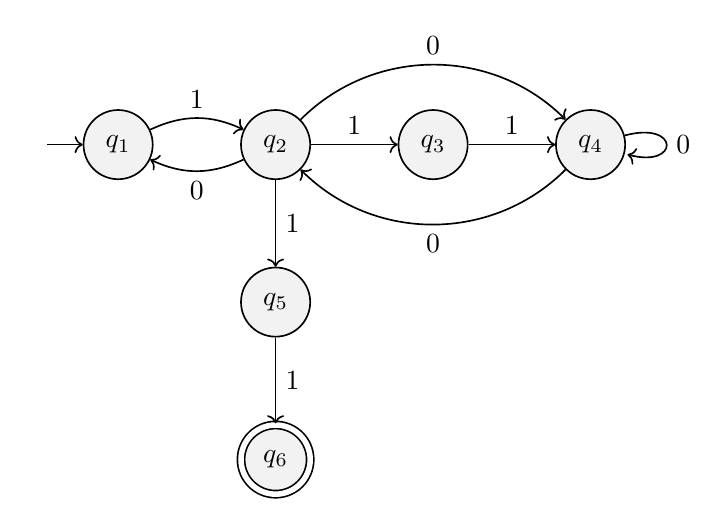
\begin{tikzpicture}
\node[state, initial] (q0) at (0,0) {$q_{1}$};
\node[state] (q1) at (2,0) {$q_{2}$};
\node[state] (q2) at (4,0) {$q_{3}$};
\node[state] (q3) at (6,0) {$q_{4}$};
\node[state] (q4) at (2,-2) {$q_{5}$};
\node[state, accepting] (q5) at (2,-4) {$q_{6}$};
\draw (q0) edge[bend left=25] node{$1$} (q1);
\draw (q1) edge[bend left=25] node{$0$} (q0);
\draw (q1) edge node{$1$} (q2);
\draw (q2) edge node{$1$} (q3);
\draw (q1) edge[bend left=45] node{$0$} (q3);
\draw (q3) edge[bend left=45] node{$0$} (q1);
\draw (q3) edge[loop right] node{$0$} (q3);
\draw (q1) edge node{$1$} (q4);
\draw (q4) edge node{$1$} (q5);
\end{tikzpicture}



\section{Left Most and Right Most Derivation in CFG}

\textbf{Definition : } a derivation $A \xrightarrow{*} \omega$ is called a left most derivation if we apply a production only to the left most variable at every step.

\textbf{Definition : } a derivation $A \xrightarrow{*} \omega$ is called a right most derivation if we apply a production only to the right most variable at every step.

\subsection{Example of left most derivation}

\begin{align*}
A &\xrightarrow{} X_{1}X_{2}X_{3} \dots X_{m} \\
&\xrightarrow{*} \omega_{1} X_{2} \dots X_{m} \\
&\xrightarrow{*} \omega_{1} \omega_{2} \dots X_{m} \\
&\xrightarrow{*} \omega_{1} \omega_{2} \dots \omega_{m} \\
\end{align*}

Thus :
\begin{align*}
A &\xrightarrow[G]{*} \omega \\
\end{align*}

\subsection{Example of right most derivation}

\begin{align*}
A &\xrightarrow{} X_{1}X_{2}X_{3} \dots X_{m} \\
&\xrightarrow{*} X_{1} X_{2} \dots \omega_{m} \\
&\xrightarrow{*} X_{1} \omega_{2} \dots \omega_{m} \\
&\xrightarrow{*} \omega_{1} \omega_{2} \dots \omega_{m} \\
\end{align*}

Thus :
\begin{align*}
A &\xrightarrow[G]{*} \omega \\
\end{align*}


\subsection{Exercise}

Consider the following Grammar :

\begin{align*}
S &\to aAS \\
S &\to a \\
A &\to SbA \\
A &\to SS \\
A &\to ba \\
\end{align*}

for input string ''aabbaa'' find :

\begin{itemize}
	\item left most derivation
	\item right most derivation
	\item derivation tree
\end{itemize}


Answer :

left most derivation :

\begin{align*}
S &\to aAS \\
&\to aSbAS \\
&\to aabAS \\
&\to aabbaS \\
&\to aabbaa \\
\end{align*}

right most derivation :

\begin{align*}
S &\to aAS \\
&\to aAa \\
&\to aSbAa \\
&\to aSbbaa \\
&\to aabbaa \\
\end{align*}

derivation tree :

\begin{tikzpicture}
\node {$S$}[sibling distance=3cm]
child {node {$a$}}
child {node {$A$}[sibling distance=2cm]
	child {node {$S$}
		child {node {$a$}}
	}
	child {node {$b$}}
	child {node {$A$}
		child {node {$b$}}
		child {node {$a$}}
	}
}
child {node {$S$}
	child {node[right] {$a$}}
};
\end{tikzpicture}


\section{Left Linear Grammar}

Left Linear Grammar :

In a Grammar if all productions are in form $A \to B\alpha$ of $A \to \alpha$ where $A, B \in V$ and $\alpha \in \Sigma^{*}$, then the gammar is called left linear grammar .

Example :

$$
A \to Aa | Bb | b
$$

\section{Right Linear Grammar}

Right Linear Grammar :

In a Grammar if all productions are in form $A \to \alpha B$ of $A \to \alpha$ where $A, B \in V$ and $\alpha \in \Sigma^{*}$, then the gammar is called right linear grammar .

Example :

$$
A \to aA | bB | b
$$

\section{Ambiguity in CFG}

\textbf{Definition :} a terminal sting $\omega \in L(G)$ is ambiguous if there exists two or more left most derivation of $\omega$ .

a CFG called G is ambiguous if there exists some $\omega \in L(G)$ which is ambiguous .

Example : 
show the grammar below is ambiguous ?

\begin{align*}
S &\to a \\
S &\to abSb \\
S &\to aAb \\
A &\to bS \\
A &\to aAAb \\
\end{align*}

Answer : you can reach the string ''abab'' with two different parse tree's so the grammar is ambiguous 

\begin{align*}
S &\to aAb \\
S &\to abSb \\
S &\to abab \\
\end{align*}

\begin{tikzpicture}
\node {$S$}[sibling distance=3cm]
child {node {$a$}}
child {node {$A$}[sibling distance=2cm]
	child {node {$b$}}
	child {node {$S$}
		child {node {$a$}}
	}
}
child {node {$b$}};
\end{tikzpicture}


\begin{align*}
S &\to abSb \\
S &\to abab \\
\end{align*}

\begin{tikzpicture}[sibling distance=3cm]
\node {$S$}
child {node {$a$}}
child {node {$b$}}
child {node {$S$}
	child {node {$a$}}
}
child {node {$b$}};
\end{tikzpicture}


\section{CFG Examples}

Let $M = (Q, \Sigma, \delta, S, F)$ be the Finite State Machine, where :

\begin{align*}
Q &= \{ A, B \} &\qquad \delta(A, a) &= A \\
\Sigma &= \{ a, b \} &\qquad \delta(A, b) &= B \\
S &= A  &\qquad \delta(B, a) &= B \\
F &= \{ B \} &\qquad \delta(B, b) &= A
\end{align*}

design a grammar to generate the language accepted by $M$ can be specified as $G=(V, \Sigma, S, P)$ where $V = Q \cup \Sigma$ and $S = A$, built the Grammar L(G) = L(M) ?


Answer :

\begin{align*}
\delta(A, a) &= A & &\Rightarrow  & A &\to aA \\
\delta(A, b) &= B & &\Rightarrow  & A &\to bB \\
\delta(B, a) &= B & &\Rightarrow  & B &\to aB \\
\delta(B, b) &= A & &\Rightarrow  & B &\to bA 
\end{align*}

$B$ is initial state $\Rightarrow B \to \wedge$
$$
\Rightarrow 
P = \{
A \to aA ,
A \to bB ,
B \to aB ,
B \to bA ,
B \to \wedge
\}
$$


\section{Simplification of Context-Free-Grammar}

In a CFG G, it may not be necessary to use all the symbols in $V \cap \Sigma$, or all the scentences in P for deriving scentences .

Sample : Consider the grammar $$G=(\{S,A,B,C,E\},\{a,b,d\},S,P)$$
where,
$$
P = \{ S \to AB, A \to a , B \to b, B \to C, E \to d | \lambda \}
$$

\begin{itemize}
	\item $C$ does not derive any terminal string
	\item $E$ and $d$ do not appear in any result
	\item $E \to \wedge$ is a null production
	\item $B \to C$ simply replace $B$ by $C$
\end{itemize}

\section{Construction of Reduced Grammar - Procedure1}

\textbf{Theorem : } If $G$ is a CFG such that $L(G) \neq \phi$, we can find an equivalent grammar $G^{\prime}$, such that each variable in $G^{\prime}$ derives some terminal string where $G=(V, \Sigma, S, P)$ and $G^{\prime} = (V^{\prime} , \Sigma, S , P^{\prime})$


\subsection{step-1 : Construction of $V^{\prime}$}

$\omega_{1}$ = \{ $A \in V | $ there exists a production $A \to \omega$ where $\omega \in \Sigma^{*}$  \}

$\omega_{i+1}$ = $\omega_{i} \cup $ \{ $A \in V | $ there exists some production $A \to \alpha$ with $\alpha \in (\Sigma \cup \omega_{i})^{*}$ \} 


$\omega_{i} \subseteq \omega_{i+1} for all i . $


\subsection{step-2 : Construction of $P^{\prime}$}

$P^{\prime}$ = \{ $A \to \alpha | $ A, $ \alpha \in (V^{\prime} \cup \Sigma)^{*}$  \}

\subsection{step-3}

for each $A \in V^{\prime}$, then $A \xrightarrow[G]{*} \omega ; \omega \in \Sigma^{*}$,

for each $A \xrightarrow[G]{*} \omega$, then $A \in V^{\prime}$ 
  
$$
L(G^{\prime}) = L(G)
$$


\subsection{Example}

Let $G = (V, \Sigma, S, P)$ be given by the productions :

\begin{align*}
S &\to AB \\
A &\to a \\
B &\to b \\
B &\to C \\
E &\to d \\
\end{align*}

Find $G^{\prime}$ derives some terminal string

Construction of $V^{\prime}$ :

$\omega_{1}$ = \{ A, B , E \} since :

\begin{align*}
A &\to a \\
B &\to b \\
E &\to d \\
\end{align*}

\begin{align*}
\omega_{2} &= \omega_{1} \cup \{ A_{1} \in V | A \to \alpha ; for \alpha \in ( \Sigma \cup \{ A, B, E \} )^{*} \} \\
&= \omega_{1} \cup \{ S \} \\
&= \{ A, B, E, S \}
\end{align*}

\begin{align*}
\omega_{3} &= \omega_{2} \cup \phi \\
&= \omega_{2} 
\end{align*}

\begin{align*}
\Rightarrow V^{\prime} = \{ A, B, E, S \}
\end{align*}

Construction of $P^{\prime}$ :

\begin{align*}
P^{\prime} &= \{ A_{1}, \alpha \in (V^{\prime} \cup \Sigma)^{*} \} \\
&= \{ S \to AB, A \to \alpha , B \to b , E \to d \}
\end{align*}


\begin{align*}
G^{\prime} &= ( \{ S, A, B, C \} , \{ a, b, c \} , S,  P^{\prime} )
\end{align*}



\subsection{Example}

Let $G = (V, \Sigma, S, P)$ be given by the productions :

\begin{align*}
S &\to AB \\
A &\to CA \\
B &\to BC \\
B &\to AB \\
A &\to a \\
C &\to aB \\
C &\to b \\
\end{align*}

Answer :

note : $\omega_{1}$ is a subset that directly derives terminal string

\begin{align*}
\omega_{1} &= \{ A, C \} 
\end{align*}

note : $\omega_{2}$ is a subset that directly derives $\omega_{1}$

\begin{align*}
\omega_{2} &= \omega_{1} \cup \{ S \} \\
&= \{ S, A, C \} 
\end{align*}

\begin{align*}
\omega_{3} &= \omega_{2} \cup \phi = \omega_{2} \\
&= \{ S, A, C \} 
\end{align*}

Thus :

\begin{align*}
\Rightarrow V^{\prime} = \{ S, A, C \}
\end{align*}

and 

\begin{align*}
\Rightarrow P^{\prime} = \{ S \to CA, A \to a, C \to b \}
\end{align*}

\section{Construction of Reduced Grammar : Procedure-2}

\textbf{Theorem : } For every CFG with Grammar $ G = (V, \Sigma, S, P)$, we can construct an equivalent Grammar $ G^{\prime} = (V^{\prime}, \Sigma^{\prime}, S, P^{\prime})$ such that every symbol in $V^{\prime} \cup \Sigma^{\prime}$ appears in some result .

Method : We construct $ G^{\prime} = (V^{\prime}, \Sigma^{\prime}, S, P^{\prime})$ as follows :

a ) Construction of $\omega_{i}$ for $i \geq 1$

\begin{align*}
\omega_{i} &= \{ S \} \\
\omega_{i+1} &= \omega_{i} \cup \{ X \in V \cup \Sigma \}
\end{align*}

$$
\omega_{i} \subseteq V \cup \Sigma
$$

$$
\omega_{i} \subseteq \omega_{i+1}
$$

b ) Construction of $V^{\prime} , \Sigma^{\prime} , P^{\prime}$

\begin{align*}
V^{\prime} &= V \cap \omega_{k} \\
\Sigma^{\prime} &= \Sigma \cap \omega_{k} \\
P^{\prime} &= \{ A \to \alpha | A \in \omega_{k} \}
\end{align*}


\subsection{Example}

Let $G = (\{ S, A, B, E \} , \{ a, b, c \}, S, P)$ where P consists of :

\begin{align*}
S &\to AB \\
A &\to a \\
B &\to b \\
E &\to d \\
\end{align*}

\begin{align*}
\omega_{1} &= \{ S \} \\
\omega_{2} &= \{ S \} \cup \{ X \in V \cup \Sigma | there \:\: exists \:\: a \:\: production \:\: A \to \alpha \:\: with \:\: A \in \omega_{i} and \:\: \alpha \:\: containing \:\: X \} \\
&= \{ S \} \cup \{ A, B \} \\
\omega_{3} &= \{ S, A, B \} \cup \{ a, b \} \\
\omega_{4} &= \omega_{3}
\end{align*}

so :

\begin{align*}
V^{\prime} &= \{ S, A, B \} \\
\Sigma^{\prime} &= \{ a, b \} \\
P^{\prime} &= \{ S \to AB , A \to a , B \to b \} \\
\end{align*}

Thus the reduced Grammar is :
$$
G^{\prime} = ( V^{\prime} , \Sigma^{\prime} , S , P^{\prime})
$$


\section{Construction of Reduced Grammar : Combining Precedure 1 and 2}

\textbf{Theorem : } For every CFG, G there exists a reduced grammar $G^{\prime}$ which is equivalent to G .

Method : We construct that reduced grammar in two steps .

step 1 : We construct a grammar G, equivalent to the grammar G, so that every variable in G, derives some terminal strings .
(i.e : the theorem steps mentioned in procedure 1)

step 2 : We construct a grammar 
$$
G^{\prime} = ( V^{\prime} , \Sigma^{\prime} , S , P^{\prime})
$$
equivalent to G, so that every symbol in $G^{\prime}$ appears in some scentence form of $G^{\prime}$ .
(i.e : the theorem steps mentioned in procedure 2)


\subsection{Example}

Construct a reduced grammar equivalent to grammar as mentioned below :

\begin{align*}
S &\to aAa \\
A &\to Sb \\
A &\to bCC \\
A &\to DaA \\
C &\to abb \\
C &\to DD \\
E &\to aC \\
D &\to aDA \\
\end{align*}


Answer :

\begin{align*}
\omega_{1} &= \{ C \}  & C &\to abb \\
\omega_{2} &= \{ C \} \cup \{ A, E \} & E &\to aC \quad A \to bCC \\
\omega_{3} &= \{ A, E, C \} \cup \{ S \} & S &\to aAa \\
\omega_{4} &= \omega_{3} \cup \phi \\
&= \{ S, A, C, E \} \\
\end{align*}

so :

\begin{align*}
P^{\prime} = \{ S \to aAa , A \to Sb , A \to bCC , C \to abb , E \to aC \}
\end{align*}

note : for the second step considered $P^{\prime}$ only .

\begin{align*}
\omega_{1} &= \{ S \}   \\
\omega_{2} &= \{ S \} \cup \{ a, A \} \\
\omega_{3} &= \{ S, A, a \} \cup \{ b, C \} \\
\omega_{4} &= \{ S, A, C, a, b \} \\
\end{align*}

$\Rightarrow$

\begin{align*}
P'' = \{ S \to aAa , A \to Sb , A \to bCC , C \to abb \}
\end{align*}

so reduced Grammar is :

$$
G = ( \{ S, A, C \} , \{ a, b \} , P'' , S )
$$


\section{Chomsky Normal Form (CNF)}

\textbf{Definition : } a CFG is in CNF, if every production is of the form $A \to a$ or $A \to BC$ and $S \to \wedge$ is in G, if $\wedge \in L(G)$, we assume that $S$ does not appear on the Right Hand Side of any production .

Example : 

If $S \to AB | \wedge$ , $A \to a$ , $B \to b$ is in G, then G is in CNF

\textbf{Theorem : } for every CFG, there is an equivalent grammar $G'$ in CNF .

\subsection{How to make some Grammar to CNF}

step1: Elimination of null and unit production .

step2 : Elimination of terminals on the Right Hand Side.

step3 : Restricting the number of variables on the Right Hand Side

\subsection{Example}

Reduce the following grammar to CNF :

G is :

\begin{align*}
S &\to aAD \\
A &\to aB | bAB \\
B &\to b \\
E &\to d \\
\end{align*}

Answer : 

step1 : There is no null and unit production.
step2 : let's create the productions according to chomsky normal form :

\begin{align*}
S &\to aAD \\
C_{a} &\to a & S &\to C_{a}AD \\
A &\to aB  \\
A &\to C_{a}B \\
A &\to bAB \\
C_{b} &\to b & A &\to C_{b}AB \\
B &\to b \\
E &\to d \\
\end{align*}

so we have :

\begin{align*}
V' &= \{ S, A, B, E, C_{a}, C_{b} \} \\
P_{1} &= \{ S \to C_{a}AD , A \to C_{a}B ,  A \to C_{b}AB , B \to b , E \to d , C_{a} \to a , C_{b} \to b \}
\end{align*}


step3 : 

\begin{align*}
S &\to C_{a}AD \\
S &\to C_{a}C_{1} \\
C_{1} &\to AD \\
A &\to C_{b}AB \\
A &\to C_{b}C_{2} \\
C_{2} &\to AB \\
\end{align*}


\subsection{Example on CNF}

Reduce the following Grammar to CNF 

G is :

\begin{align*}
S &\to aAbB \\
A &\to aA \\
A &\to a \\
B &\to bB \\
B &\to b \\
\end{align*}

step2 :

\begin{align*}
S &\to aAbB & C_{a} &\to a & C_{b} &\to b \\
S &\to C_{a}AC_{b}B \\
A &\to aA & A &\to C_{a}A \\
B &\to bB & B &\to C_{b}B \\
\end{align*}

step3 :

\begin{align*}
S &\to C_{a}AC_{b}B \\
S &\to C_{a}C_{1} \\
C_{1} &\to AC_{b}B \\
C_{1} &\to AC_{2} \\
C_{2} &\to C_{b}B \\
\end{align*}

so G is :

\begin{align*}
V &= \{ A, B, S, C_{a}, C_{b}, C_{1}, C_{2} \} \\
\Sigma &= \{ a, b \} \\
S &= start state \\
\end{align*}

and P is :
P = \{ 
\begin{align*}
A &\to a \\
B &\to b \\
C_{a} &\to a \\ 
C_{b} &\to b \\ 
A &\to C_{a}A \\ 
B &\to C_{b}B \\ 
S &\to C_{a}C_{1} \\ 
C_{1} &\to AC_{b}B \\ 
C_{1} &\to AC_{2} \\
C_{b} &\to C_{b}B  \\
\end{align*}
\} 

\section{Greibach Normal Form}

a CFG is in GNF if every production is of form :

$$
A \to a\alpha
$$

where $\alpha \in V^{*}$ and $\alpha \in \Sigma$ , $S \to \wedge$ is allowed in G, if $\wedge \in L(G)$, we assume that S does not appear on the Right Hand Side of any production .

Example : 

a grammar G with following production rules is in GNF :

\begin{align*}
S &\to b \\
S &\to aBC \\
S &\to \wedge \\
B &\to bBC \\
C &\to c \\
B &\to b 
\end{align*}



\chapter{Push Down Automata}

\section{Definition of Push Down Automata}

\textbf{Definition :} a PDA is a 7-tuple $A = (Q,\Sigma,\Gamma,\delta,q_{0},Z_{0},F)$ where :

\begin{itemize}
	\item a finite non-empty set of states denoted by $Q$
	\item a finite non-empty set of input symbols denoted by $\Sigma$
	\item a finite non-empty set of push down symbols denoted by $\Gamma$
	\item a special state $q_{0}$, called initial state, where $q_{0} \in Q$
	\item a special push down symbols called initial symbol on the push down store denoted by $Z_{0}$
	\item the set of final states, a subset of $Q$ denoted by $F$
	\item the transition function $\delta$ from $Q \times (\Sigma \times \{\lambda\}) \times \Gamma$ to the set if finite subsets of $Q \times \Gamma^{*}$
	$$
	Q \times (\Sigma \times \{\lambda\}) \times \Gamma \to Q \times \Gamma^{*}
	$$
\end{itemize}


\subsection{Example}

Design a PDA 
$$
A = (Q,\Sigma,\Gamma,\delta,q_{0},Z_{0},F)
$$
which accepts input strings over ''a'' \& ''b'', but the input string should contain even number of a's .

Sample : abbaabab

Answer :

$$
\delta = 
\begin{cases}
\delta(\overbrace{q_{0}}^{state},\overbrace{a}^{input},\overbrace{Z_{0}}^{stack-top}) = (q_{0}, aZ_{0}) \\
\delta(q_{0},a,a) = (q_{0},\wedge) \\
\delta(q_{0},b,a) = (q_{0},a) \\
\delta(q_{0},b,Z_{0}) = (q_{0},Z_{0}) \\
\delta(q_{0},\wedge,Z_{0}) = (q_{f},Z_{0}) \\
\end{cases}
$$

note : reaching to final state means the string is accepted

so :

\begin{align*}
Q &= \{ q_{0}, q_{f} \} \\
\Sigma &= \{ a, b \} \\
\Gamma &= \{ Z_{0}, a \} \\
F &= \{ q_{f} \} 
\end{align*}


\section{PDA : Accepting of a string}

\begin{itemize}
	\item Acceptance by Final state
	\item Acceptance by Null Store
\end{itemize}

\subsection{Definition 1 - Acceptance by Final state}

Let 
$$
A = (Q,\Sigma,\Gamma,\delta,q_{0},Z_{0},F)
$$
be a PDA, The set accepted by PDA by final state is defined by 
$$
T(A) = \{ \omega \in \Sigma^{*} | (q_{0},\omega,Z_{0}) \vdash (q_{f}, \wedge, \alpha ) for \: some \: q_{f} \in F \:\: and \:\: \alpha \in \tau^{*}  \}
$$

\subsection{Definition 2 - Acceptance by Null Store}

Let 
$$
A = (Q,\Sigma,\tau,\delta,q_{0},Z_{0},F)
$$
be a PDA, The set accepted by PDA by null state ( or empty store ) is defined by 
$$
N(A) = \{ \omega \in \Sigma^{*} | (q_{0},\omega,Z_{0}) \vdash^{*} (q, \wedge, \wedge ) for \: some \: q \in Q \}
$$


\section{PDA to Context-Free-Grammars}

\textbf{Theorem :} if L is a CFL, then we can construct a PDA A accepting L by empty store, i.e : N(A)

Method : Let $L = L(G)$, where $G=(V, \Sigma, S, P)$ is a Context-Free-Grammar, we construct a PDA A as
$$
A = (\{ q \},\Sigma, V \cup \Sigma ,\delta,q,S,\phi)
$$
where $\delta$ is defined by the following rules :
\begin{align*}
R_{1} &: \delta(q,\wedge,A) = \{ (q,\alpha) | A \to \alpha \:\: is \:\: in \:\: P \} \\
R_{2} &: \delta(q_{1},a,a) = \{ (q,\wedge) | for \:\: every \:\: a \:\: in \:\: \Sigma \} \\
\end{align*}


\subsection{Example}

Construct a PDA which is equivalent to the following CFG :
\begin{align*}
S &\to 0CC \\
C &\to 0S \\
C &\to 1S \\
C &\to 0 \\
\end{align*}

test whether 010*{4} is accepted by N(A) ?

Solution :

$\delta$ is defined by the following rules :

\begin{align*}
R_{1} :  \delta(q,\wedge,S) &= \{ (q,0CC) \} \\
  \delta(q,\wedge,C) &= \{ (q,0S), (q,1S), (q,0) \} \\
R_{2} : \delta(q,1,1) &= \{ (q,\wedge) \} \\
 \delta(q,0,0) &= \{ (q,\wedge) \} \\
\end{align*}

so : 

\begin{align*}
(q, 010^{4}, S) &\vdash (q, 010^{4}, 0CC) \\
&\vdash (q, 10^{4}, CC) \\
&\vdash (q, 10^{4}, 1SC) \\
&\vdash (q, 0^{4}, SC) \\
&\vdash (q, 0^{4}, 0CCC) \\
&\vdash (q, 0^{3}, CCC) \\
&\vdash (q, 0^{3}, 0CC) \\
&\vdash (q, 0^{2}, CC) \\
&\vdash (q, 0^{2}, 0C) \\
&\vdash (q, 0, C) \\
&\vdash (q, 0, 0) \\
&\vdash (q, \wedge, \wedge) \\
\end{align*}

So $010^{4} \in N(A)$


\subsection{Example}

Design a PDA which accepts
$$
T(A) = \{ \omega \in \omega^{T} | where \:\: \omega \in (a,b)^{+} \}
$$

sample :
$$
\underbrace{abb}_{\omega}c\underbrace{bba}_{\omega^{T}}
$$


Answer :

$$
\delta = 
\begin{cases}
\delta(q_{0},a,Z_{0}) = (q_{0}, aZ_{0}) \\
\delta(q_{0},b,Z_{0}) = (q_{0},bZ_{0}) \\
\delta(q_{0},a,a) = (q_{0},aa) \\
\delta(q_{0},a,b) = (q_{0},ab) \\
\delta(q_{0},b,a) = (q_{0},ba) \\
\delta(q_{0},b,b) = (q_{0},bb) \\
\delta(q_{0},c,a) = (q_{1},a) \\
\delta(q_{0},c,b) = (q_{1},b) \\
\delta(q_{1},a,a) = (q_{1},\wedge) \\
\delta(q_{1},b,b) = (q_{1},\wedge) \\
\delta(q_{1},\wedge,Z_{0}) = (q_{f},Z_{0}) \\
\end{cases}
$$


\subsection{Example}

Design a PDA which accepts 
$$
T(A) = \{ a^{n} b^{n} | n > 0 \}
$$

sample : if n = 3 $\to$ $\omega$ = aaabbb


Answer :

$$
\delta = 
\begin{cases}
\delta(q_{0},a,Z_{0}) = (q_{0}, aZ_{0}) \\
\delta(q_{0},a,a) = (q_{0},aa) \\
\delta(q_{0},b,a) = (q_{1},\wedge) \\
\delta(q_{1},b,a) = (q_{1},\wedge) \\
\delta(q_{0},\wedge,Z_{0}) = (q_{f},Z_{0}) \\
\end{cases}
$$




\subsection{Example}

Design a PDA which accepts 
$$
N(A) = \{ a^{n} b^{m}a^{n} | n, m \geq 1 \}
$$

note : N(A) means Null-Terminating .

sample : $\underbrace{aaa}_{q_{0}}\underbrace{bb}_{q_{1}}\underbrace{aaa}_{q_{2}}$


Answer :

$$
\delta = 
\begin{cases}
\delta(q_{0},a,Z_{0}) = (q_{0}, aZ_{0}) \\
\delta(q_{0},a,a) = (q_{0},aa) \\
\delta(q_{0},b,a) = (q_{1},a) \\
\delta(q_{1},b,a) = (q_{1},a) \\
\delta(q_{1},a,a) = (q_{2},\wedge) \\
\delta(q_{2},a,a) = (q_{2},\wedge) \\
\delta(q_{2},\wedge,Z_{0}) = (q_{2},\wedge) \\
\end{cases}
$$



\subsection{Example}

Design a PDA which accepts 
$$
N(A) = \{ a^{n} b^{2n} | n \geq 1 \}
$$

note : for every a we should push two a at top of the stack .


Answer :

$$
\delta = 
\begin{cases}
\delta(q_{0},a,Z_{0}) = (q_{0}, aaZ_{0}) \\
\delta(q_{0},a,a) = (q_{0},aaa) \\
\delta(q_{0},b,a) = (q_{1},\wedge) \\
\delta(q_{1},b,a) = (q_{1},\wedge) \\
\delta(q_{1},\wedge,Z_{0}) = (q_{1},\wedge) \\
\end{cases}
$$





\subsection{Example}

Design a PDA which accepts 
$$
N(A) = \{ a^{m} b^{m} c^{n} | m, n \geq 1 \}
$$



Answer :

$$
\delta = 
\begin{cases}
\delta(q_{0},a,Z_{0}) = (q_{0}, aZ_{0}) \\
\delta(q_{0},a,a) = (q_{0},aa) \\
\delta(q_{0},b,a) = (q_{1},\wedge) \\
\delta(q_{1},b,a) = (q_{1},\wedge) \\
\delta(q_{1},\wedge,Z_{0}) = (q_{1},\wedge) \\
\end{cases}
$$

note : we don't care how many times we see 'c' .



\subsection{Example}

Design a PDA which accepts 
$$
N(A) = \{ a^{m} b^{n} | m > n \geq 1 \}
$$

note : because $m > n$ , the stack should remain 'a' at top of the stack

Answer :

$$
\delta = 
\begin{cases}
\delta(q_{0},a,Z_{0}) = (q_{0}, aZ_{0}) \\
\delta(q_{0},a,a) = (q_{0},aa) \\
\delta(q_{0},b,a) = (q_{1},\wedge) \\
\delta(q_{1},b,a) = (q_{1},\wedge) \\
\delta(q_{1},\wedge,a) = (q_{2},\wedge) \\
\delta(q_{2},\wedge,a) = (q_{2},\wedge) \\
\delta(q_{2},\wedge,Z_{0}) = (q_{2}, \wedge) \\
\end{cases}
$$


\section{LL(K) Grammar}

suppose LL(1) Grammar :

First L $\xrightarrow{means}$ Reading input string from left to right

Second L  $\xrightarrow{means}$ Left Most Derivation

1 $\xrightarrow{means}$ looking ahead terminal symbols in the input string



\chapter{Turing Machine}

\section{Turing Machine}

\textbf{Definition :} a Turing Machine, M is a 7-tuple $(Q ,\Sigma , \Gamma , \delta , q_{0} , b , F)$ where :

\begin{itemize}
	\item $Q$ is a finite non-empty set of states.
	\item $\Gamma$ is a finite non-empty set of tape symbols.
	\item $b \in \Gamma$ is the blank.
	\item $\Sigma$ is a finite non-empty set of input symbols . $\Sigma$ is a subset of $\Gamma$ and $b \notin \Sigma$ .
	\item $\delta$ is the transition function mapping the states of finite automaton and tape symbols and movement of the head .
	
	i.e : $Q \times \Gamma \to Q \times \Gamma \times \{ L , R \}$
	\item $q_{0} \in Q$ is the initial state.
	\item $F \subseteq Q$ is the set of final states.
\end{itemize}


* The acceptability of a string is decided by the reachability from the initial state to same final state, so final states are also called as accepting states .

* $\delta$ may not be defined for some elements of $Q \times \Gamma$


\begin{center}
	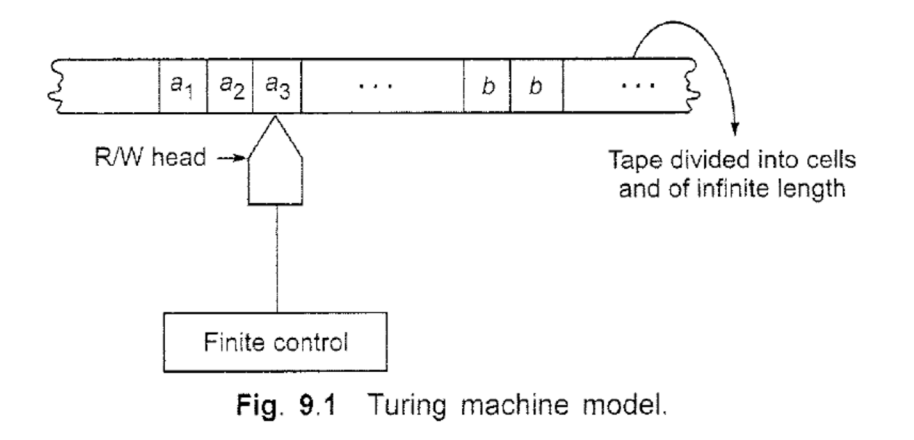
\includegraphics[scale=.7]{./turing.png}
	%\caption{}
\end{center}

* Tape devided into cells containing tape symbols .

* Head can move left or right .



\section{Turing Maching : Instanteneous Description (ID)}
\textbf{Definition : } ID of a Turing Machine, is a snapshot of TM to describe the current situation of the TM .

\subsection{Transitions}

let the initial ID of a TM is 

$$
x_{1} x_{2} \dots x_{i-1} \underbrace{x_{i}}_{q} x_{i+1} \dots x_{n}
$$

So :

$$
x_{1} x_{2} \dots x_{i-1} \underbrace{x_{i}}_{q} x_{i+1} \dots x_{n} \xrightarrow{\delta(q,x_{i}) = (p,y,L)}  x_{1} x_{2} \dots \underbrace{x_{i-1}}_{p} y x_{i+1} \dots x_{n}
$$


$$
x_{1} x_{2} \dots x_{i-1} \underbrace{x_{i}}_{q} x_{i+1} \dots x_{n} \xrightarrow{\delta(q,x_{i}) = (p,y,R)}  x_{1} x_{2} \dots  x_{i-1} y \underbrace{x_{i+1}}_{p} \dots x_{n}
$$


\section{TM : Aceptance through transition Table}


\begin{tabular}{ r | l l l l l  } 
     & $0$ & $1$ & $x$ & $y$ & $b$  \\
\hline
$\to q_{1}$ & $xRq_{2}$ & $-$ & $-$ &$-$ & $bRq_{5}$\\
$q_{2}$ & $0Rq_{2}$ & $yLq_{3}$ & $-$ & $yRq_{2}$ & $-$ \\
$q_{3}$ & $0Lq_{4}$ & $-$ & $xRq_{5}$ & $yLq_{3}$ & $-$  \\
$q_{4}$ & $0Lq_{4}$ & $-$ & $xRq_{1}$ & $-$ & $-$   \\
$q_{5}$ & $-$ & $-$ & $-$ & $yRq_{5}$ & $bRq_{6}$   \\
$(f) q_{6}$ & $-$ & $-$ & $-$ & $-$ & $-$   \\
\end{tabular}

check wether input string $0011$ is accepted or not by the given turing machine shown above ?

Answer :

\begin{align*}
 \underbrace{0}_{q_{1}}011 &\vdash x\underbrace{0}_{q_{2}}11 \\
 &\vdash x0\underbrace{1}_{q_{2}}1 \\
 &\vdash x\underbrace{0}_{q_{3}}y1 \\
 &\vdash \underbrace{x}_{q_{4}}0y1 \\
 &\vdash x\underbrace{0}_{q_{1}}y1 \\
 &\vdash xx\underbrace{y}_{q_{2}}1 \\
 &\vdash xxy\underbrace{1}_{q_{2}} \\
 &\vdash xx\underbrace{y}_{q_{3}}y \\
 &\vdash x\underbrace{x}_{q_{3}}yy \\
 &\vdash xx\underbrace{y}_{q_{5}}y \\
 &\vdash xxy\underbrace{y}_{q_{5}} \\
 &\vdash xxyy\underbrace{b}_{q_{5}} \\
 &\vdash xxyyb\underbrace{b}_{q_{6}} \\
\end{align*}


* $q_{6}$ is the final state so the string is accepted .


\section{ TM : Acceptance through transition system }


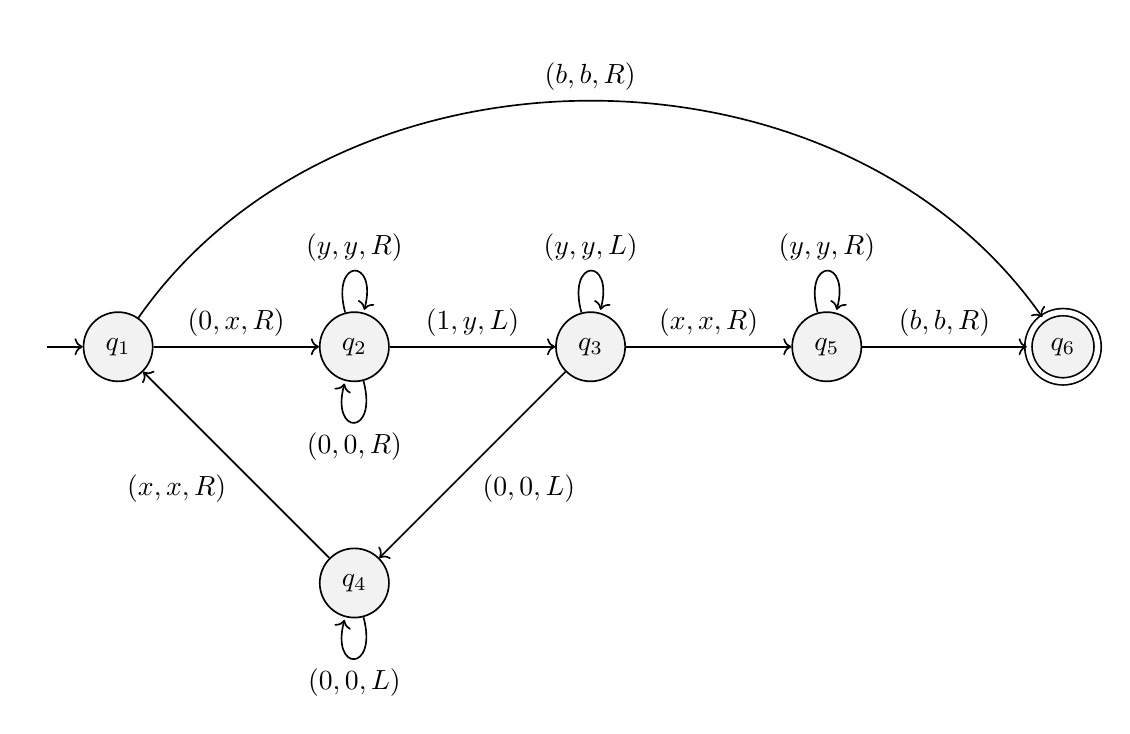
\begin{tikzpicture}
\node[state, initial] (q1) at (0,0) {$q_{1}$};
\node[state] (q2) at (3,0) {$q_{2}$};
\node[state] (q3) at (6,0) {$q_{3}$};
\node[state] (q4) at (3,-3) {$q_{4}$};
\node[state] (q5) at (9,0) {$q_{5}$};
\node[state, accepting] (q6) at (12,0) {$q_{6}$};
\draw (q1) edge node{$(0,x,R)$} (q2);
\draw (q2) edge[loop above] node{$(y,y,R)$} (q2);
\draw (q2) edge[loop below] node{$(0,0,R)$} (q2);
\draw (q2) edge node{$(1,y,L)$} (q3);
\draw (q3) edge[loop above] node{$(y,y,L)$} (q3);
\draw (q3) edge node{$(0,0,L)$} (q4);
\draw (q4) edge node{$(x,x,R)$} (q1);
\draw (q4) edge[loop below] node{$(0,0,L)$} (q4);
\draw (q3) edge node{$(x,x,R)$} (q5);
\draw (q5) edge[loop above] node{$(y,y,R)$} (q5);
\draw (q5) edge node{$(b,b,R)$} (q6);
\draw (q1) edge[bend left=55]node{$(b,b,R)$} (q6);
\end{tikzpicture}



check the above TM accepts input string $0011$ or not ?

Answer :

\begin{align*}
\underbrace{0}_{q_{1}}011 &\xrightarrow{(0,x,R)} x\underbrace{0}_{q_{2}}11 \\
&\xrightarrow{(0,0,R)} x0\underbrace{1}_{q_{2}}1 \\
&\xrightarrow{(1,y,L)} x\underbrace{0}_{q_{3}}y1 \\
&\xrightarrow{(0,0,L)} \underbrace{x}_{q_{4}}0y1 \\
&\xrightarrow{(x,x,R)} x\underbrace{0}_{q_{1}}y1 \\
&\xrightarrow{(0,x,R)} xx\underbrace{y}_{q_{2}}1 \\
&\xrightarrow{(y,y,R)} xxy\underbrace{1}_{q_{2}} \\
&\xrightarrow{(1,y,L)} xx\underbrace{y}_{q_{3}}y \\
&\xrightarrow{(y,y,L)} x\underbrace{x}_{q_{3}}yy \\
&\xrightarrow{(x,x,R)} xx\underbrace{y}_{q_{5}}y \\
&\xrightarrow{(y,y,R)} xxy\underbrace{y}_{q_{5}} \\
&\xrightarrow{(y,y,R)} xxyy\underbrace{b}_{q_{5}} \\
&\xrightarrow{(b,b,R)} xxyyb\underbrace{b}_{q_{6}} \\
\end{align*}



* $q_{6}$ is the final state so the TM accepts the string .



\subsection{Example}
TM : 1's complement of a binary number 

result :

$$
b01101b \xrightarrow[TM]{*} b10010b
$$


\begin{tabular}{r | c c c  } 
& \multicolumn{3}{ c }{Tape Symbols}  \\
        & $0$ & $1$ & $b$  \\
\hline
$\to q_{0}$ & $1Rq_{0}$ & $0Rq_{0}$ & $bLq_{1}$ \\
$q_{1}$ & $0Lq_{1}$ & $1Lq_{1}$ & $bRq_{f}$ \\
$q_{f}$ & $-$ & $-$ & $-$ \\
\end{tabular}

* The Machine HALT at $q_{f}$




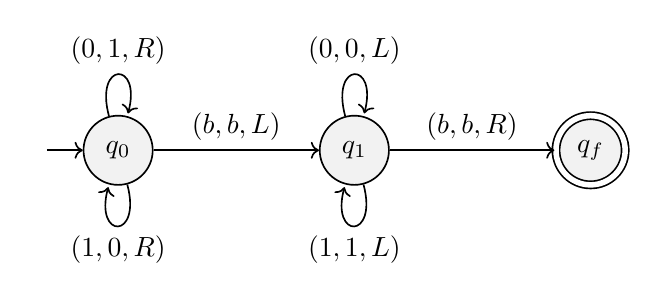
\begin{tikzpicture}
\node[state, initial] (q1) at (0,0) {$q_{0}$};
\node[state] (q2) at (3,0) {$q_{1}$};
\node[state, accepting] (qf) at (6,0) {$q_{f}$};
\draw (q1) edge[loop above] node{$(0,1,R)$} (q1);
\draw (q1) edge[loop below] node{$(1,0,R)$} (q1);
\draw (q1) edge node{$(b,b,L)$} (q2);
\draw (q2) edge[loop above] node{$(0,0,L)$} (q2);
\draw (q2) edge[loop below] node{$(1,1,L)$} (q2);
\draw (q2) edge node{$(b,b,R)$} (qf);
\end{tikzpicture}




\section{Example}

TM : Even number of 0's and Odd number of 1's .\\\\
EE $\xrightarrow{means}$ Even number of 0's and Even number of 1's \\
OE $\xrightarrow{means}$ Odd number of 0's and Even number of 1's \\
OO $\xrightarrow{means}$ Odd number of 0's and Odd number of 1's \\
EO $\xrightarrow{means}$ Even number of 0's and Odd number of 1's \\

\begin{align*}
EE &\to q_{0} \\ 
OE &\to q_{1} \\ 
OO &\to q_{2} \\ 
EO &\to q_{f} \\ 
\end{align*}

\begin{tabular}{ l r | c c c  } 
& \multicolumn{3}{ c }{Tape Symbols}  \\
        & $0$ & $1$ & $b$  \\
\hline
EE & $\to q_{0}$ & $0Rq_{1}$ & $1Rq_{f}$ & $-$ \\
OE & $q_{1}$ & $0Rq_{0}$ & $1Rq_{2}$ & $-$ \\
OO & $q_{2}$ & $0Rq_{f}$ & $1Rq_{1}$ & $-$ \\
EO & $q_{f}$ & $0Rq_{2}$ & $1Rq_{0}$ & $-$ \\
\end{tabular}


\end{document}